% Chapter Template

\chapter{Conception} % Main chapter title

\label{Chapter2} % Change X to a consecutive number; for referencing this chapter elsewhere, use \ref{ChapterX}

\lhead{Chapitre 2. \emph{Conception}} % Change X to a consecutive number; this is for the header on each page - perhaps a shortened title

%----------------------------------------------------------------------------------------
%	SECTION 1
%----------------------------------------------------------------------------------------

\section{Description textuelle structurée des cas d'utilisation}

%-----------------------------------
%	SUBSECTION 1
%-----------------------------------
\subsection{Se connecter au système}
\begin{enumerate}
\item Scénario de base 
\begin{enumerate}
\item Le Superviseur se connecte, en tant que tel, en remplissant le formulaire de connexion présent sur la page d’accueil puis en cliquant sur le bouton “Se connecter”.

\end{enumerate}
\item Extensions
\begin{enumerate}
\item Erreur de connexion

\begin{enumerate}
\item Message d’erreur et retour à l’étape 1 du scénario de base.
\end{enumerate}
\end{enumerate}
\end{enumerate}

\subsection{Charger le plan d'une zone}
\begin{enumerate}
\item Précondition
\begin{enumerate}
\item 
Se connecter au Système
\end{enumerate}


\item Scénario de base
\begin{enumerate}
\item Erreur de connexion
\item Le Système indique le niveau de chargement du fichier grâce à une petite icône de chargement.
\item Le Système valide la conformité du fichier en affichant une icône de validation verte.
\item Le système affiche le plan chargé dans l’espace prévu
\end{enumerate}

\item Extensions
\begin{description}
\item [Chargement interrompu] Le Système indique l’échec du chargement : croix rouge + message d’erreur : ”Erreur de chargement du fichier, veuillez recommencer”
\item [Fichier incorrect : erreur rédhibitoire] Traitement interrompu et affichage d’erreur :  croix rouge accompagnée du message d’erreur correspondant.
\item [Fichier incorrect : erreur acceptable]
Le traitement du fichier continue mais un message explique l’erreur et en conséquence ce qui n’a pas été chargé 
\end{description}
\end{enumerate}

%-----------------------------------
%	SUBSECTION 2
%-----------------------------------

\subsection{Charger et calculer une demande de livraisons}
\begin{enumerate}
\item Précondition
\begin{enumerate}
\item Se connecter au Système + Charger plan d’une zone géographique
\end{enumerate}


\item Scénario de base
\begin{enumerate}
\item Le Superviseur clique sur le menu Fichier puis le sous-menu “Charger les demandes de livraison” puis va chercher le fichier correspondant.  
\item Le Système indique le niveau de chargement du fichier grâce à une petite icône de chargement.
\item Le Système valide la conformité du fichier en affichant une icône de validation verte.
\item Le système met à jour l’affichage du plan avec une première proposition de chemin ?
\item Le Système affiche plusieurs nouvelles sections. Une section plan contenant les tournées, des boutons “annuler”, “refaire”, zoom “+” et dézoom “-”.  Une section “Information sur le noeud sélectionné” contenant au départ un texte : “Cliquez sur un point de livraison pour afficher ses informations” et une section ayant le bouton “Générer la feuille de route”.

\end{enumerate}

\item Extensions
\begin{description}
\item [Chargement interrompu] Le Système indique l’échec du chargement : croix rouge + message d’erreur :”Erreur de chargement, veuillez recommencer”.
\item [Fichier incorrect : erreur rédhibitoire] Traitement interrompu et affichage d’erreur :  croix rouge accompagnée du message d’erreur correspondant.
\item [Fichier incorrect : erreur acceptable] Le traitement du fichier continue mais un message explique l’erreur et en conséquence ce qui n’a pas été chargé.
\item [Une tournée calculée contient des problèmes] Le Système indique le problème par un point d'exclamation sur le plan, au niveau du point correspondant.
\end{description}
\end{enumerate}

\subsection{Modifier une tournée la veille}
\begin{enumerate}
\item Précondition
\begin{enumerate}
\item Se connecter au Système + Charger plan d’une zone géographique + Charger et calculer les demandes de livraison du lendemain
\end{enumerate}

\item Scénario de base : Suppression d'un point
\begin{enumerate}
\item Le Superviseur clique sur un point de livraison de la tournée puis clique sur le bouton “Supprimer”.
\item Le Système calcule le chemin le plus court entre les points précédent et suivant du point supprimé.
\item Le Système met à jour l’affichage du plan.
\item Le Système dégrise le bouton Annuler qui est dans le menu Édition.

\end{enumerate}

\item Scénario de base : Insertion d'un point
\begin{enumerate}
\item Le Superviseur clique sur un nœud.
\item Le Système affiche “Cliquez sur le point suivant votre nouveau point de livraison”.
\item Le Superviseur clique le point suivant le nouveau point de livraison.
Le Système calcule le chemin le plus court entre le point ajouté et le point le précédent puis entre le point ajouté et le point le suivant.
\item Le Système met à jour l’affichage du plan.
\item Le Système dégrise le bouton Annuler qui est dans le menu Édition

\end{enumerate}
\item Extensions
\begin{enumerate}
\item Le Superviseur clique que sur un nœud mais ne clique pas ensuite sur un point de livraison.
\begin{enumerate}
\item Le nœud ne devient pas un point de livraison.
\end{enumerate}
\end{enumerate}
\end{enumerate}

\subsection{Annuler des modifications}
\begin{enumerate}
\item Précondition
\begin{enumerate}
\item Avoir modifié au moins une fois la tournée, avoir fini un des scénarios de base.
\end{enumerate}


\item Scénario de base : Annuler insertion
\begin{enumerate}
\item Le Superviseur clique sur le menu Edition puis le sous-menu “Annuler”.
\item Le Système supprime le point dernièrement crée.
\item Le Système met à jour l’affichage du plan.
\item Le Système grise le bouton Annuler si il n’y a plus d’actions à annuler.


\end{enumerate}
\item Scénario de base : Annuler suppression
\begin{enumerate}
\item Le Système recrée le point dernièrement supprimer et recalcule la tournée.
\item Le Système met à jour l’affichage du plan.
\item Le Système grise le bouton Annuler si il n’y a plus d’actions à annuler.
\end{enumerate}
\end{enumerate}




\subsection{Refaire des modifications}
\begin{enumerate}
\item Précondition
\begin{enumerate}
\item Avoir annulé une opération.
\end{enumerate}


\item Scénario de base : Annuler dernière opération

\end{enumerate}
\subsection{Générer une feuille de route}

\begin{enumerate}
\item Précondition
\begin{enumerate}
\item Se connecter au Système + Charger plan d’une zone géographique + Charger les demandes de livraison du lendemain + Générer une tournée

\end{enumerate}


\item Scénario de base 
\begin{enumerate}
\item Le Superviseur clique sur le bouton “Générer la feuille de route”.
\item Le Système édite une version txt de l’ensemble des feuilles de route. 
\end{enumerate}
\end{enumerate}




%----------------------------------------------------------------------------------------
%	SECTION 2
%----------------------------------------------------------------------------------------
\clearpage
\section{Diagrammes de packages et de classes}
\subsection{Package model}
\begin{figure}[H]
\centering
	\centering
		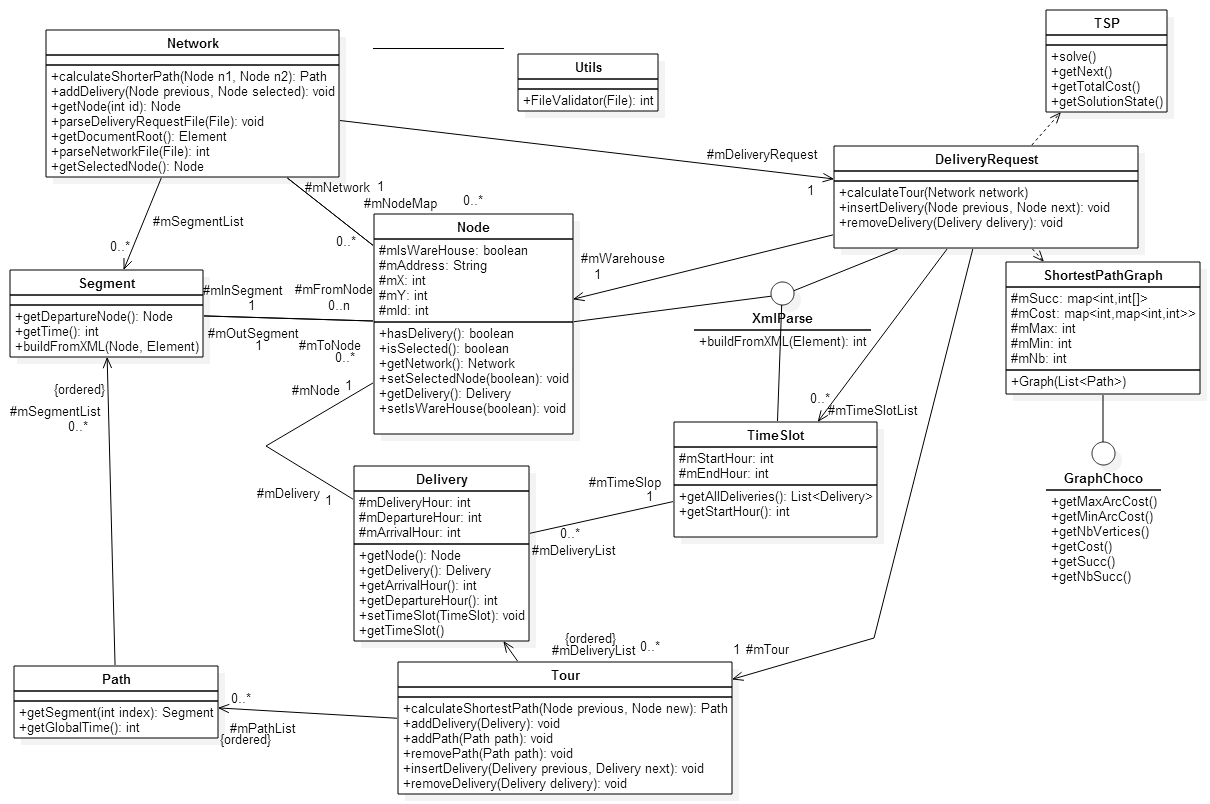
\includegraphics[width=\textwidth,height=\textheight,keepaspectratio, angle=90]{Figures/modele}
		\rule{35em}{0.5pt}
	\caption[Model]{Package Model}
\end{figure}

\subsection{Package view}
\begin{figure}[H]
	\centering
		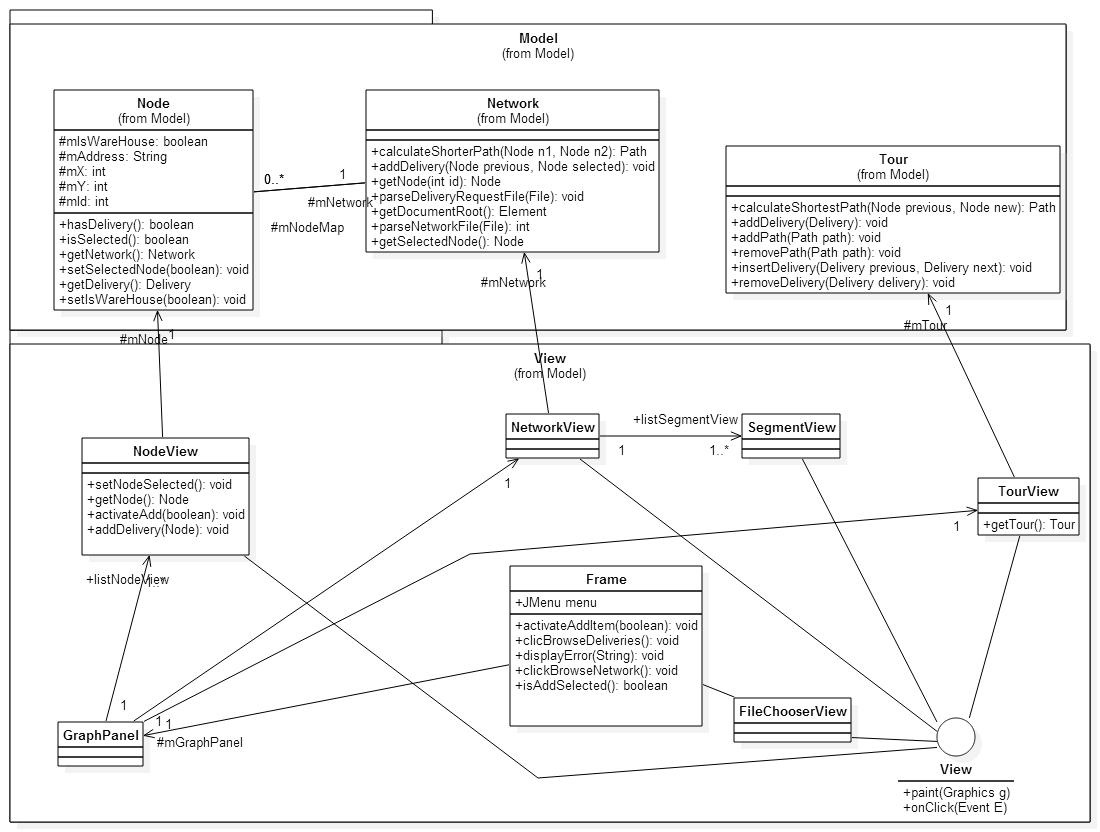
\includegraphics[width=\textwidth,height=\textheight,keepaspectratio, angle=90]{Figures/vue}
		\rule{35em}{0.5pt}
	\caption[View]{Package View}
\end{figure}

\subsection{Package controller}
\begin{figure}[H]
	\centering
		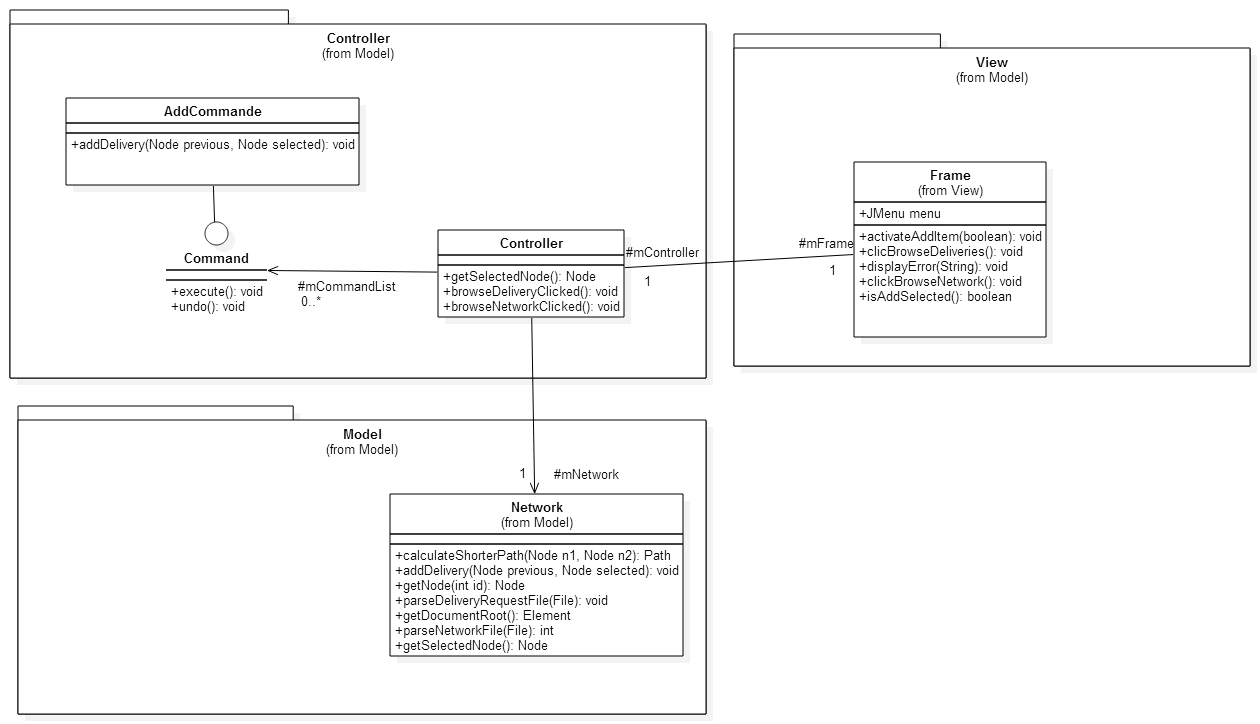
\includegraphics[width=\textwidth,height=\textheight,keepaspectratio, angle=90]{Figures/controleur}
		\rule{35em}{0.5pt}
	\caption[Controller]{Package Controller}
\end{figure}


\section{Diagrammes de séquence}

\subsection{Chargement du plan d'une zone}
\begin{figure}[H]
	\centering
		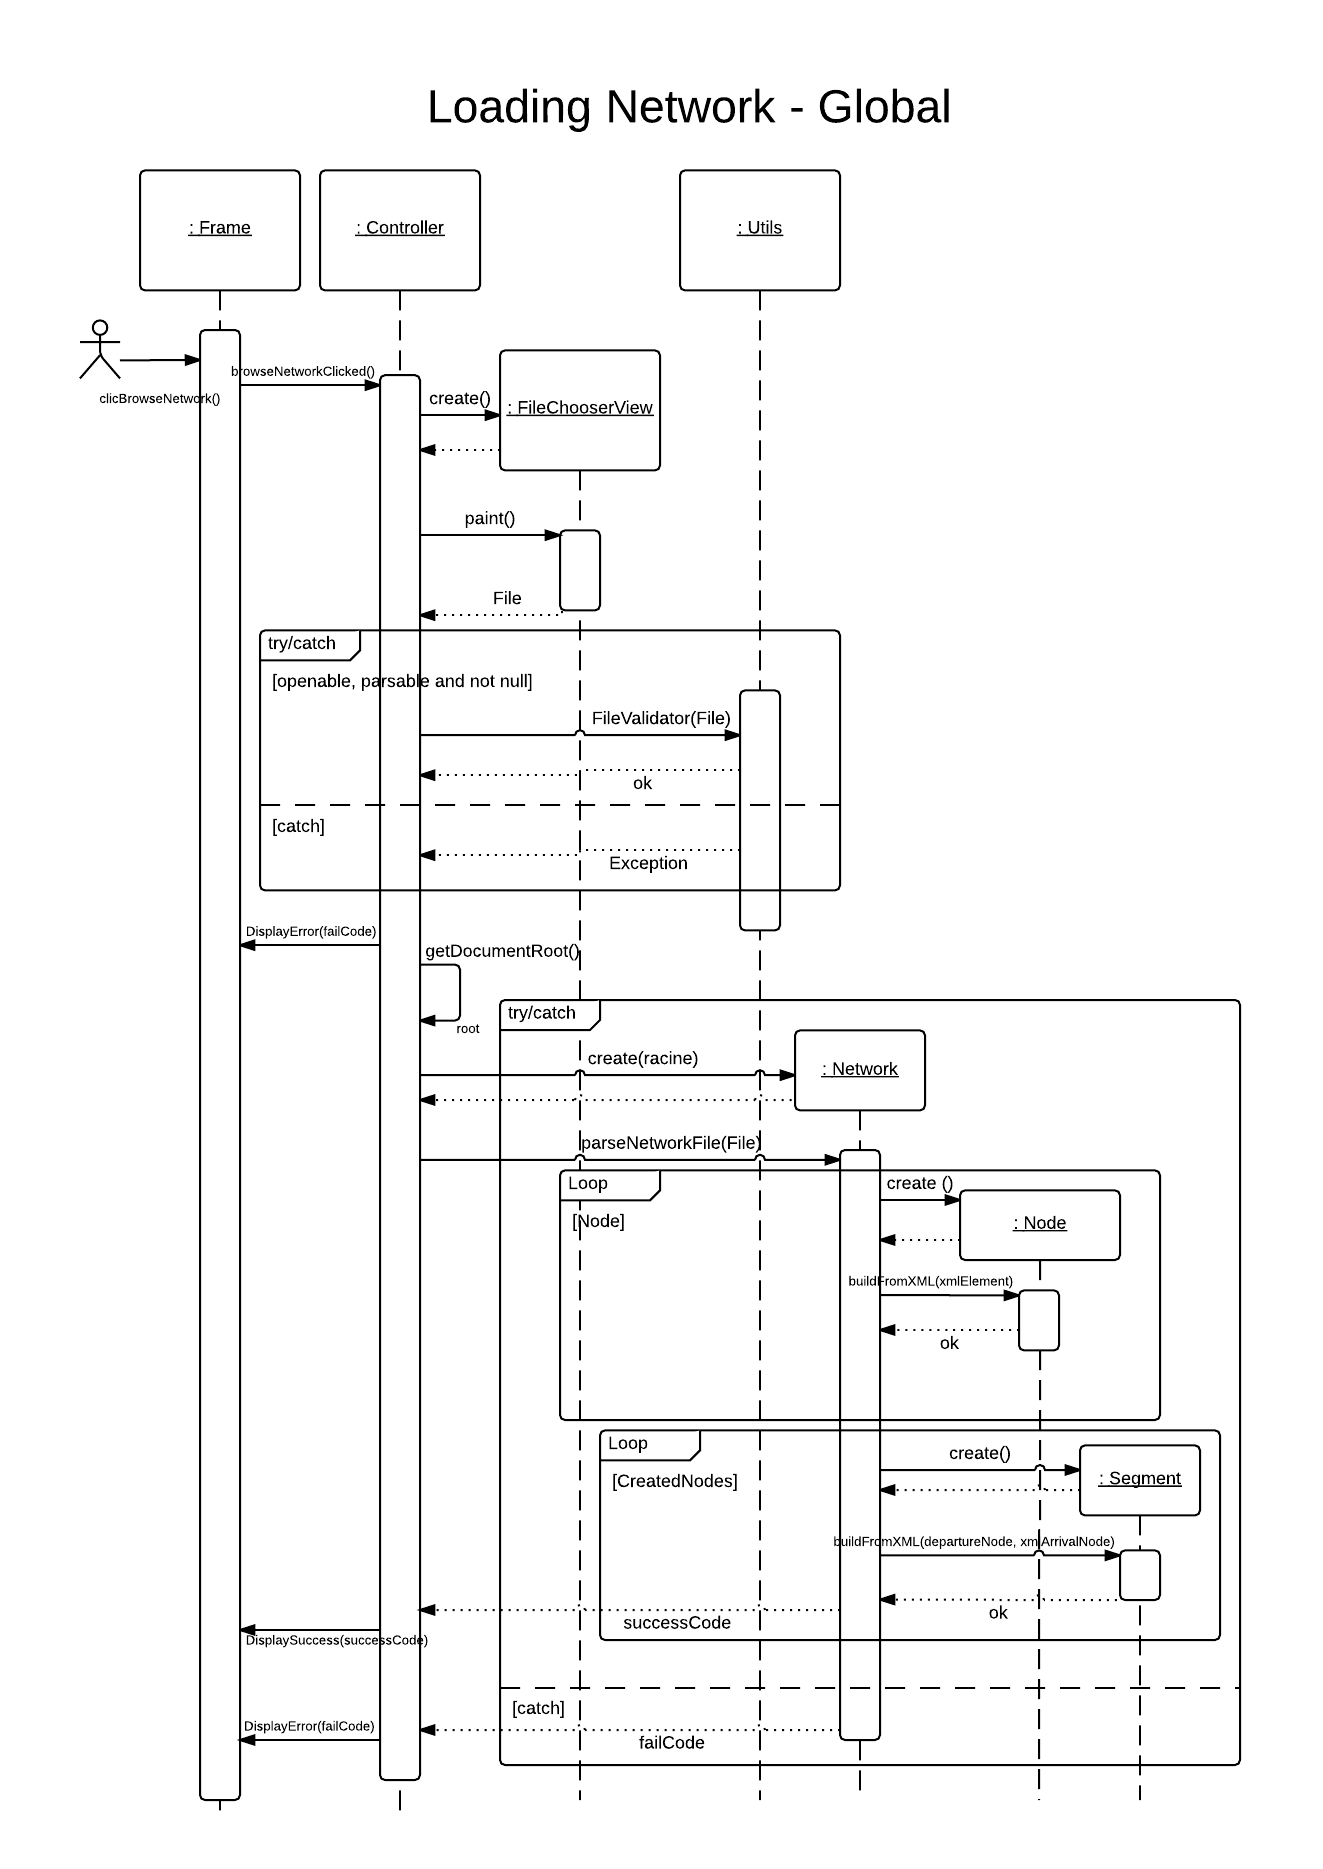
\includegraphics[width=\textwidth,height=\textheight,keepaspectratio]{Figures/plan_zone}
		\rule{35em}{0.5pt}
	\caption[Chargement du plan d'une zone]{Chargement du plan d'une zone}
\end{figure}

\subsection{Chargement d'une demande de livraison}
\begin{figure}[H]
	\centering
		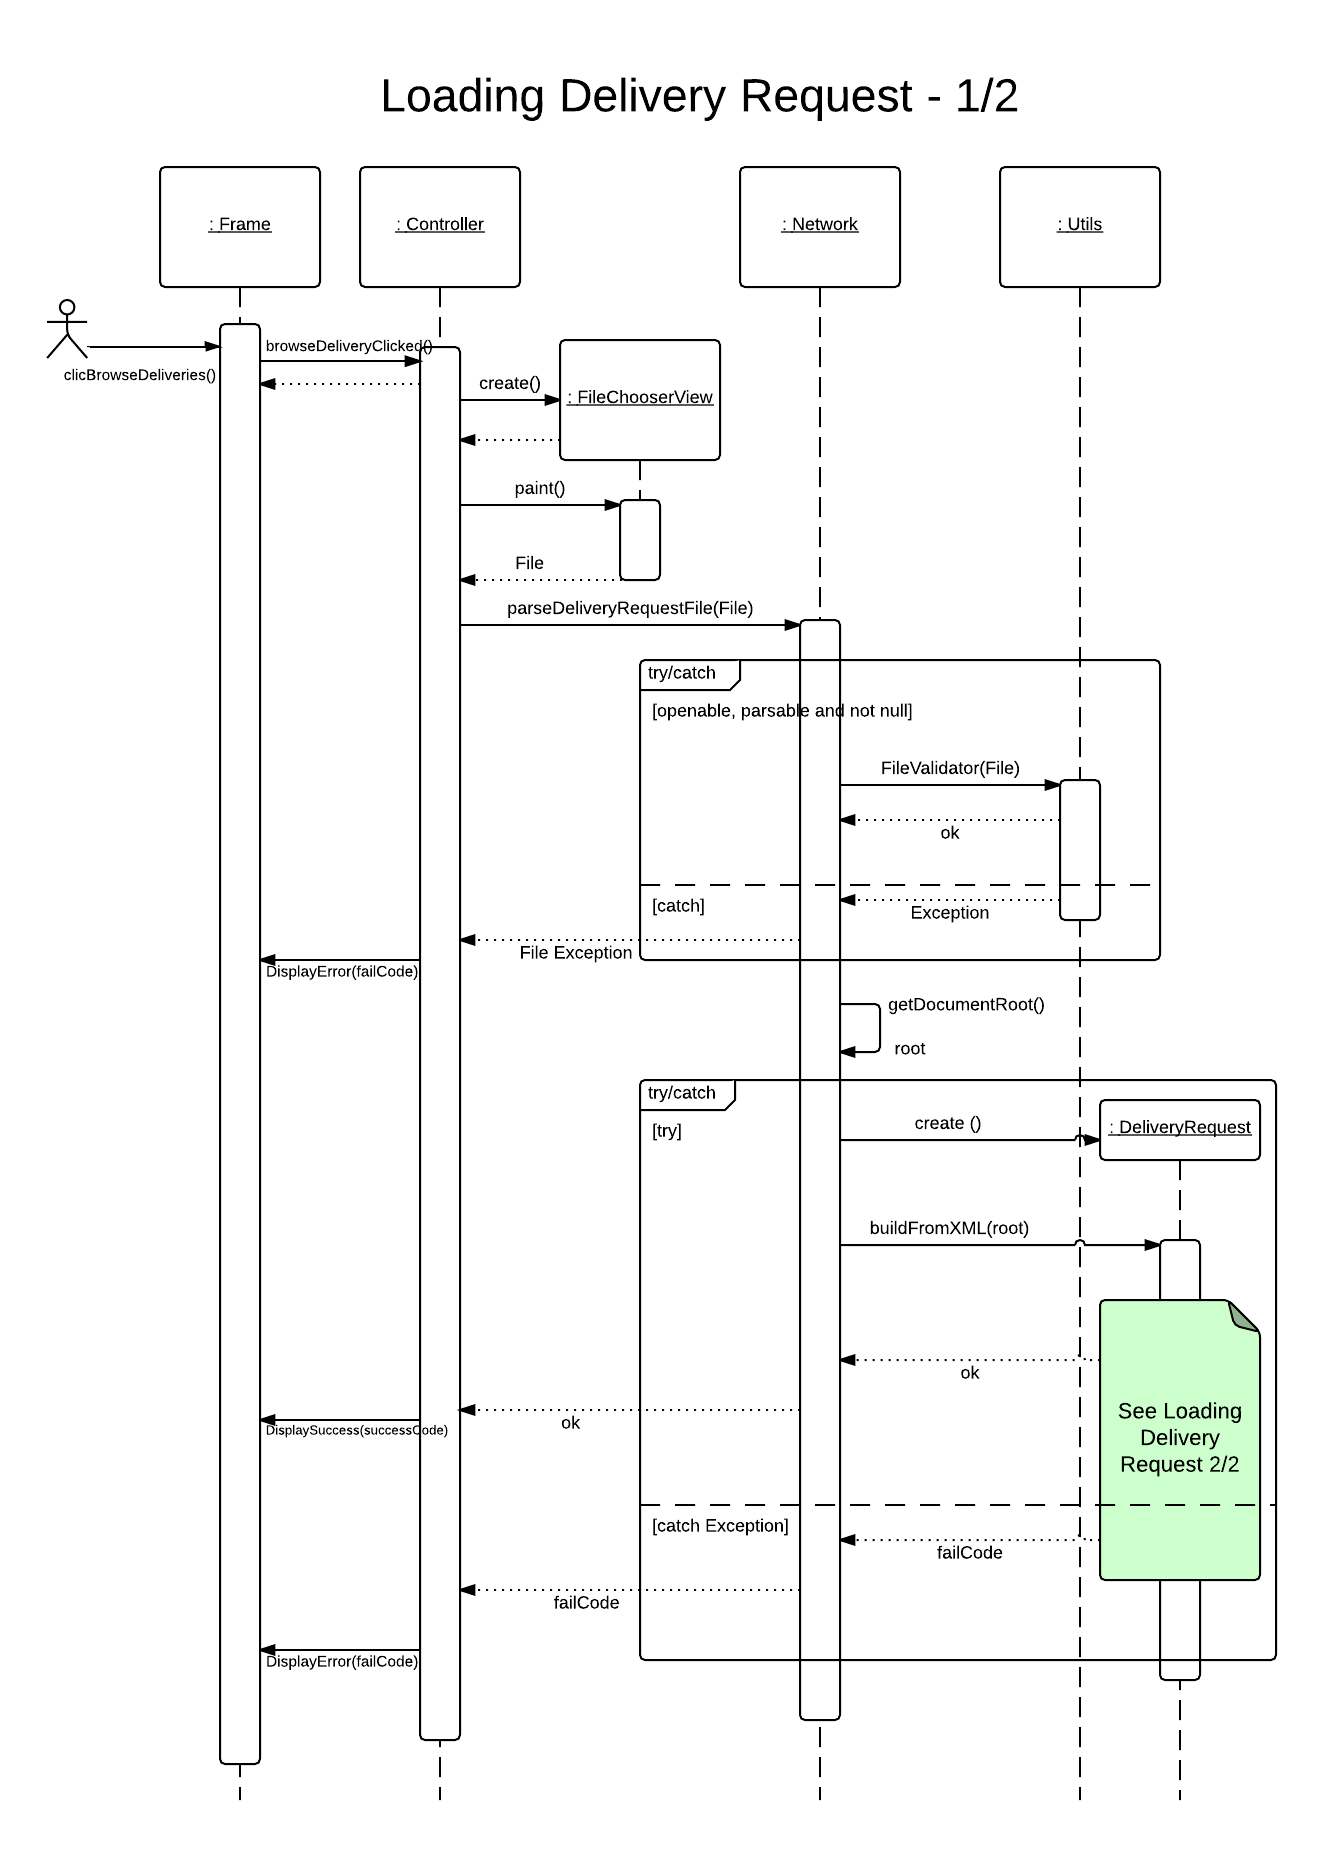
\includegraphics[width=\textwidth,height=\textheight,keepaspectratio]{Figures/chargement1}
		\rule{35em}{0.5pt}
	\caption[Chargement d'une demande de livraison - Partie 1]{Chargement d'une demande de livraison - Partie 1}
\end{figure}

\begin{figure}[H]
	\centering
		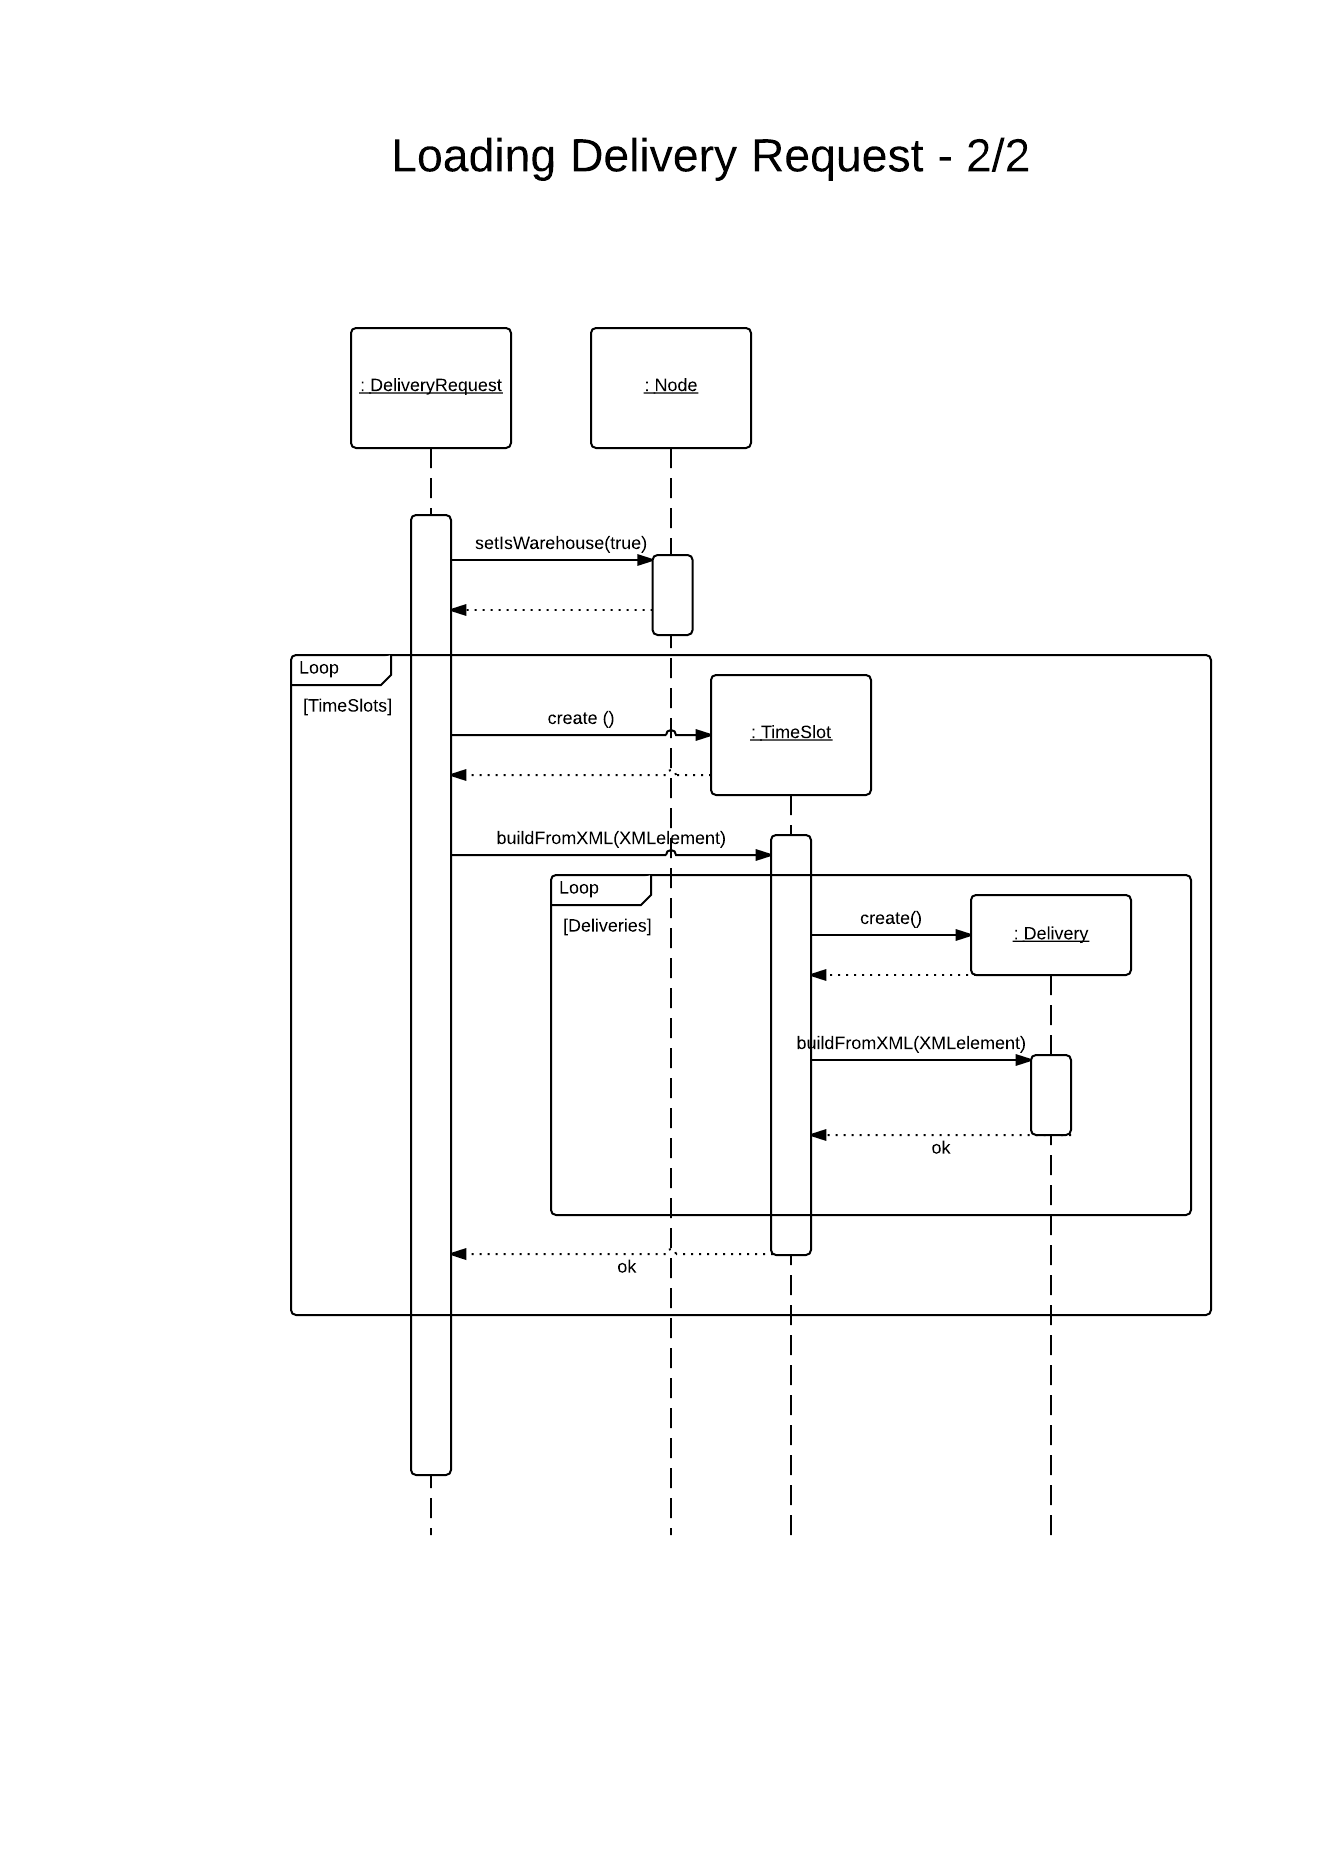
\includegraphics[width=\textwidth,height=\textheight,keepaspectratio]{Figures/chargement2}
		\rule{35em}{0.5pt}
	\caption[Chargement d'une demande de livraison - Partie 2]{Chargement d'une demande de livraison - Partie 2}
\end{figure}

\subsection{Calcul d'une tournée}
\begin{figure}[H]
	\centering
		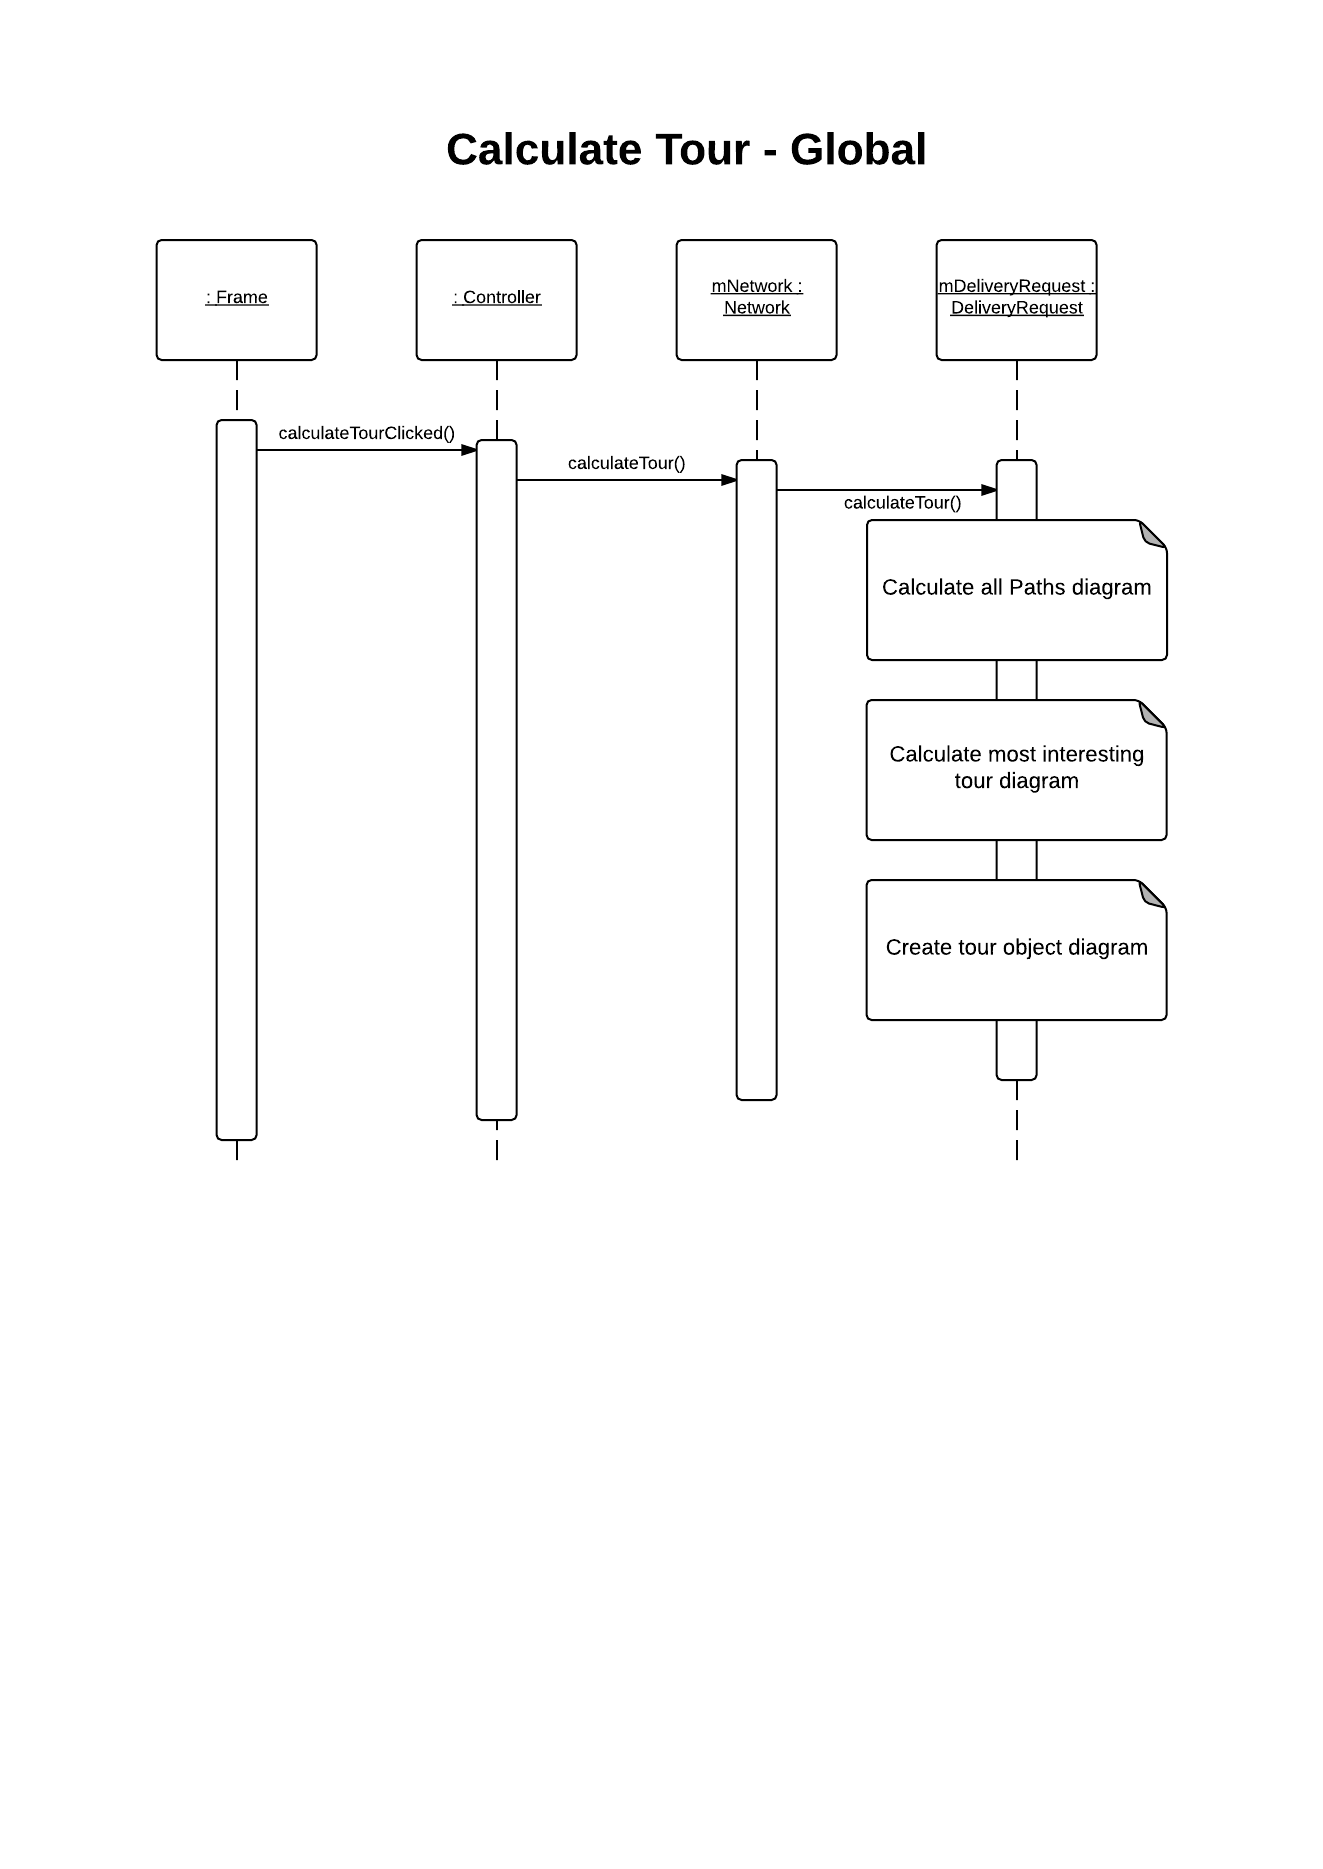
\includegraphics[width=\textwidth,height=\textheight,keepaspectratio]{Figures/calcul_tournee1}
		\rule{35em}{0.5pt}
	\caption[Calcul d'une tournée-général]{Calcul d'une tournée-général}
\end{figure}

\begin{figure}[H]
	\centering
		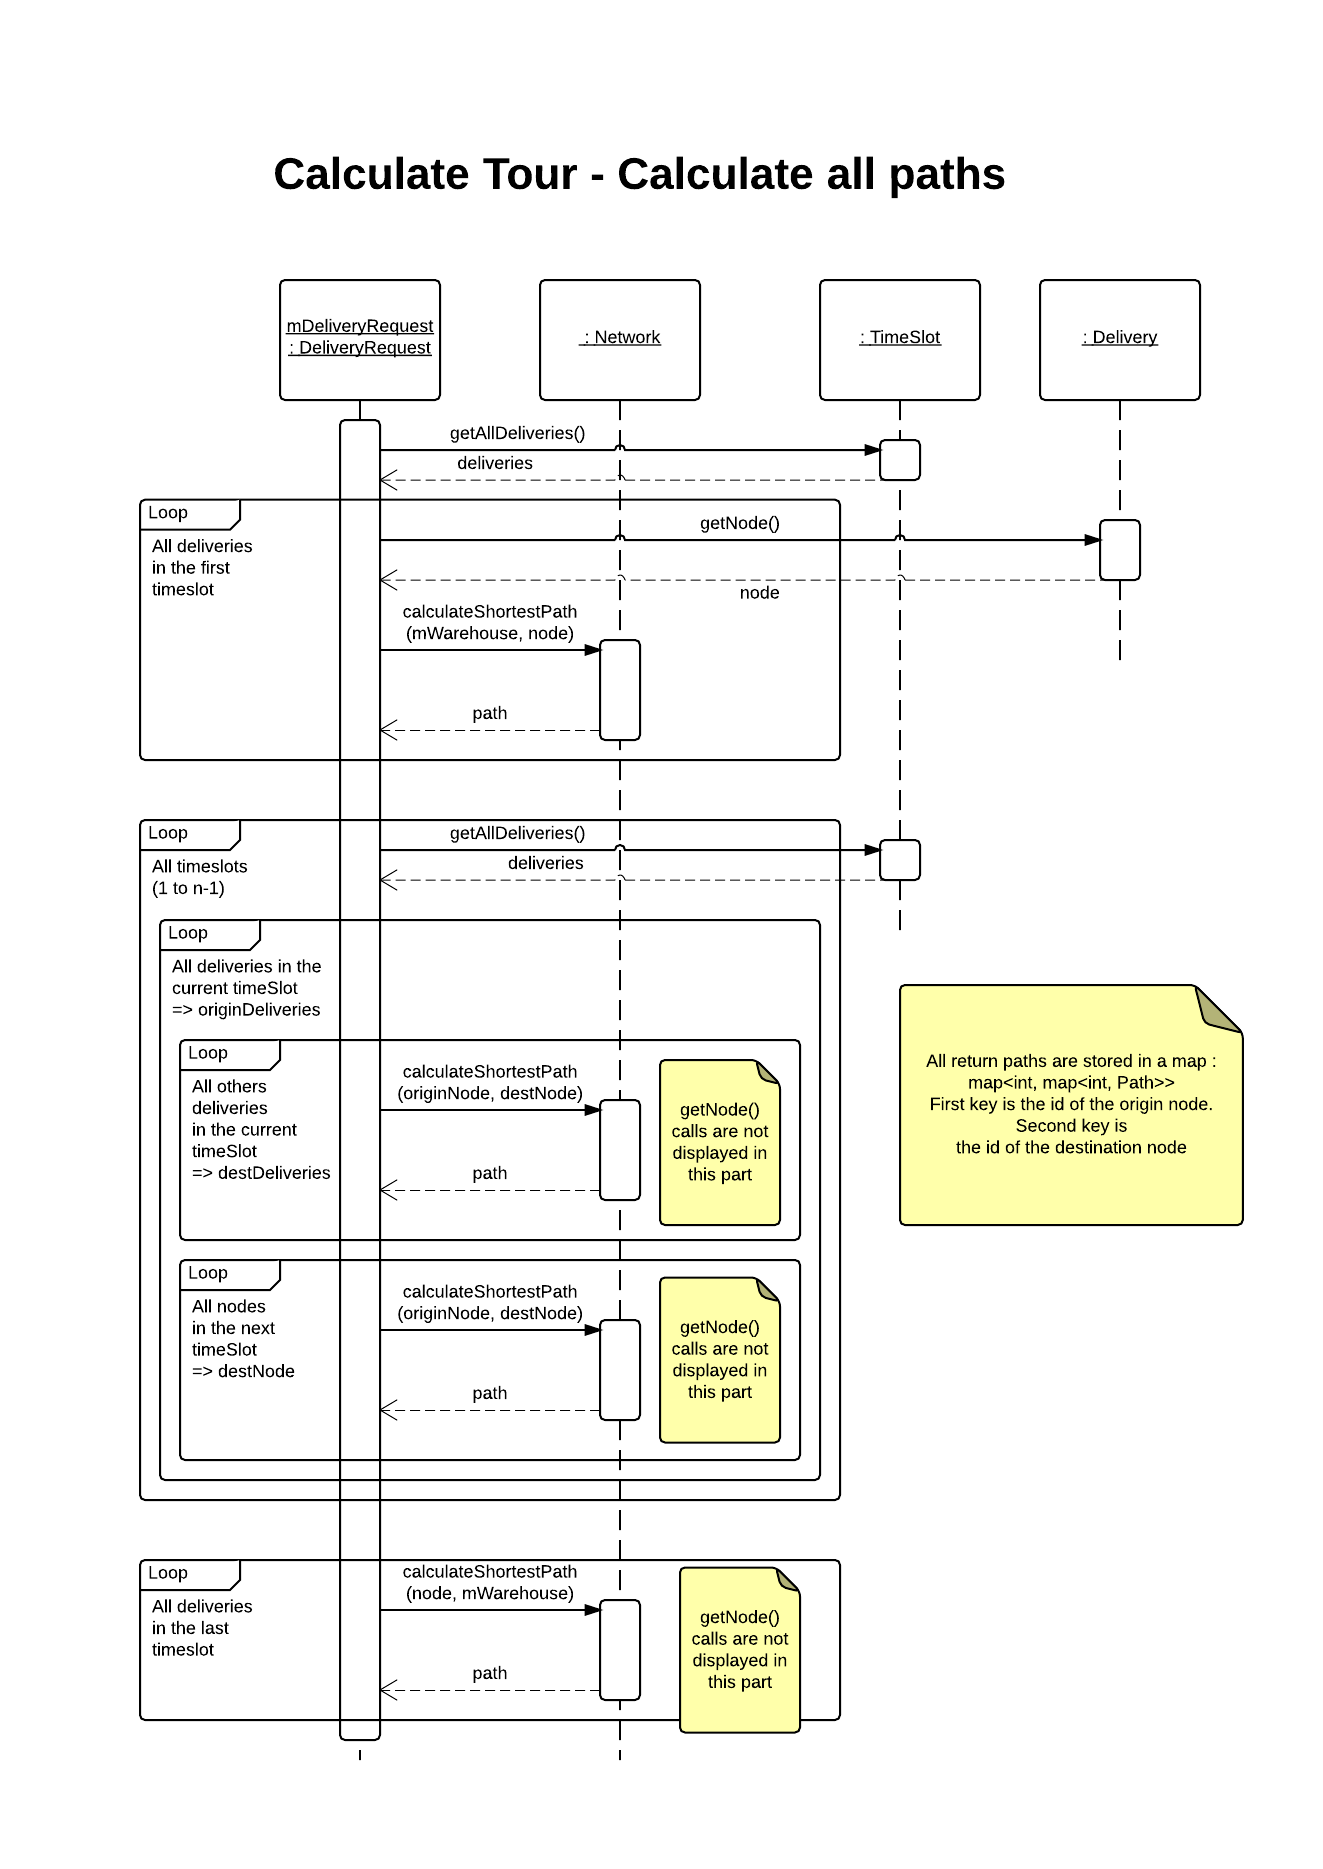
\includegraphics[width=\textwidth,height=\textheight,keepaspectratio]{Figures/calcul_tournee2}
		\rule{35em}{0.5pt}
	\caption[Calcul des plus courts chemins]{Calcul des plus courts chemins}
\end{figure}

\begin{figure}[H]
	\centering
		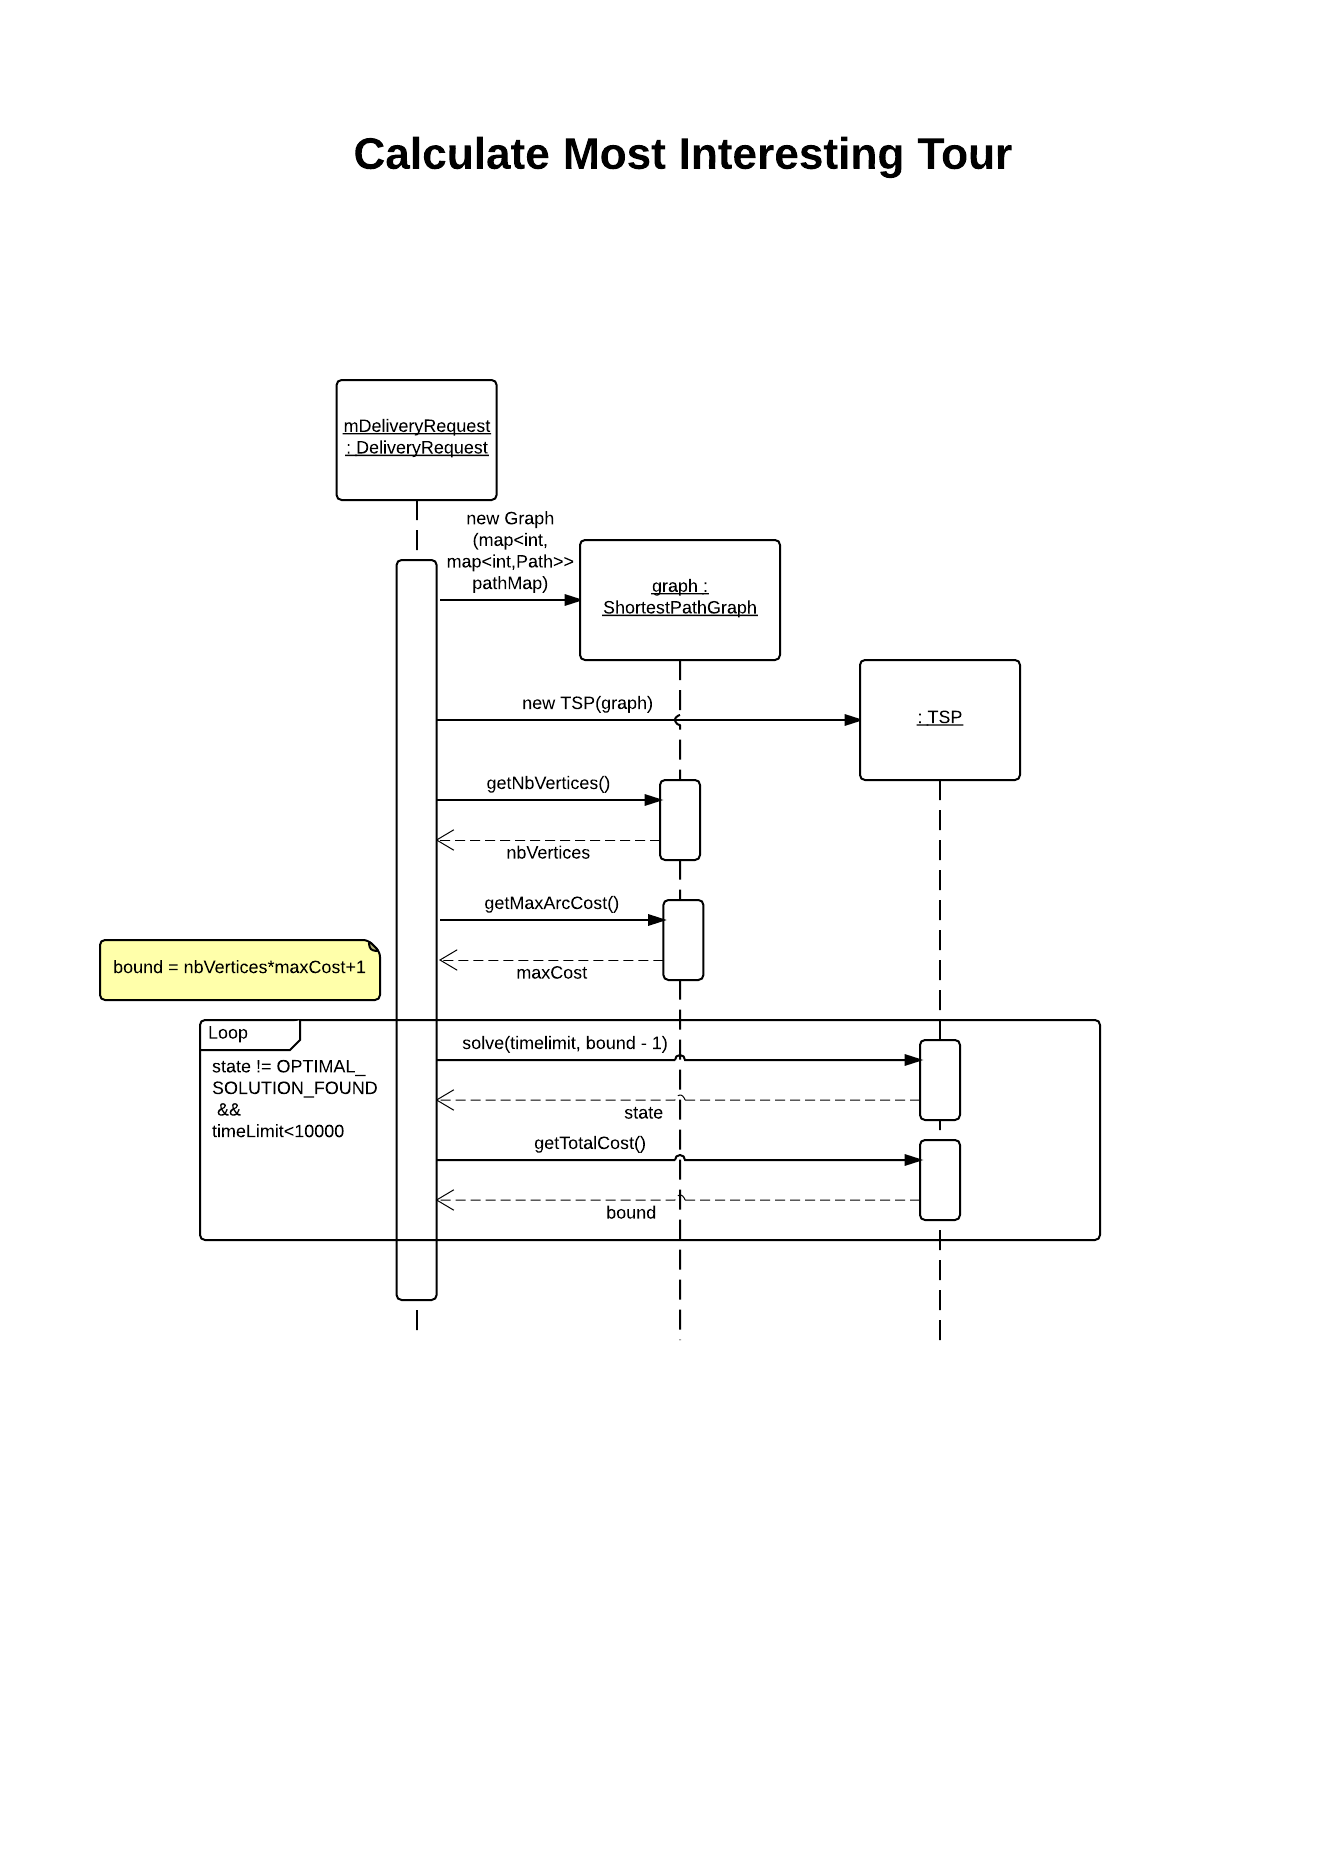
\includegraphics[width=\textwidth,height=\textheight,keepaspectratio]{Figures/calcul_tournee3}
		\rule{35em}{0.5pt}
	\caption[Calcul de la tournée la plus intéressante]{Calcul de la tournée la plus intéressante}
\end{figure}

\begin{figure}[H]
	\centering
		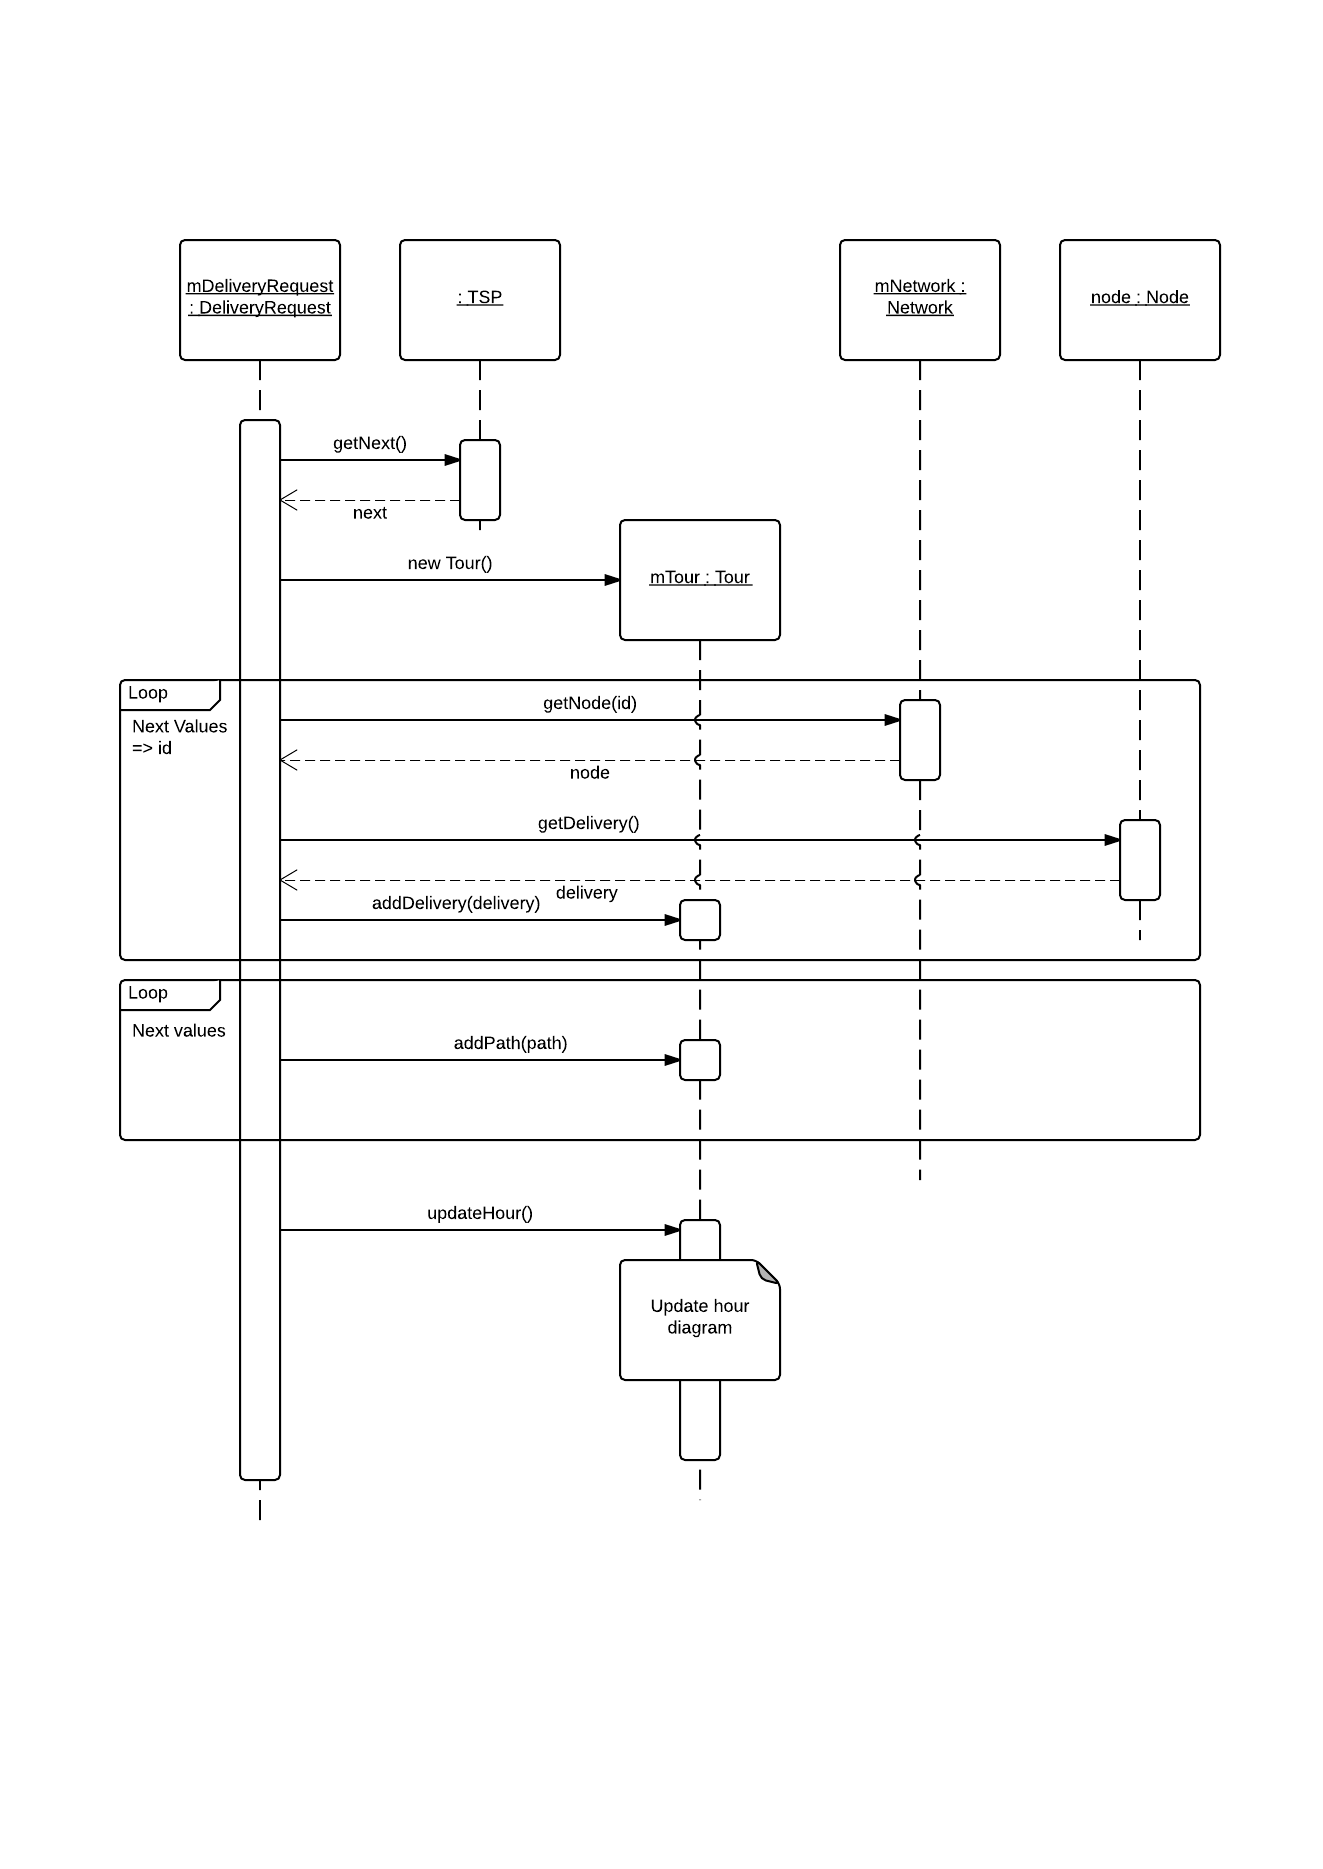
\includegraphics[width=\textwidth,height=\textheight,keepaspectratio]{Figures/calcul_tournee4}
		\rule{35em}{0.5pt}
	\caption[Construction de l'itinéraire]{Construction de l'itinéraire}
\end{figure}

\begin{figure}[H]
	\centering
		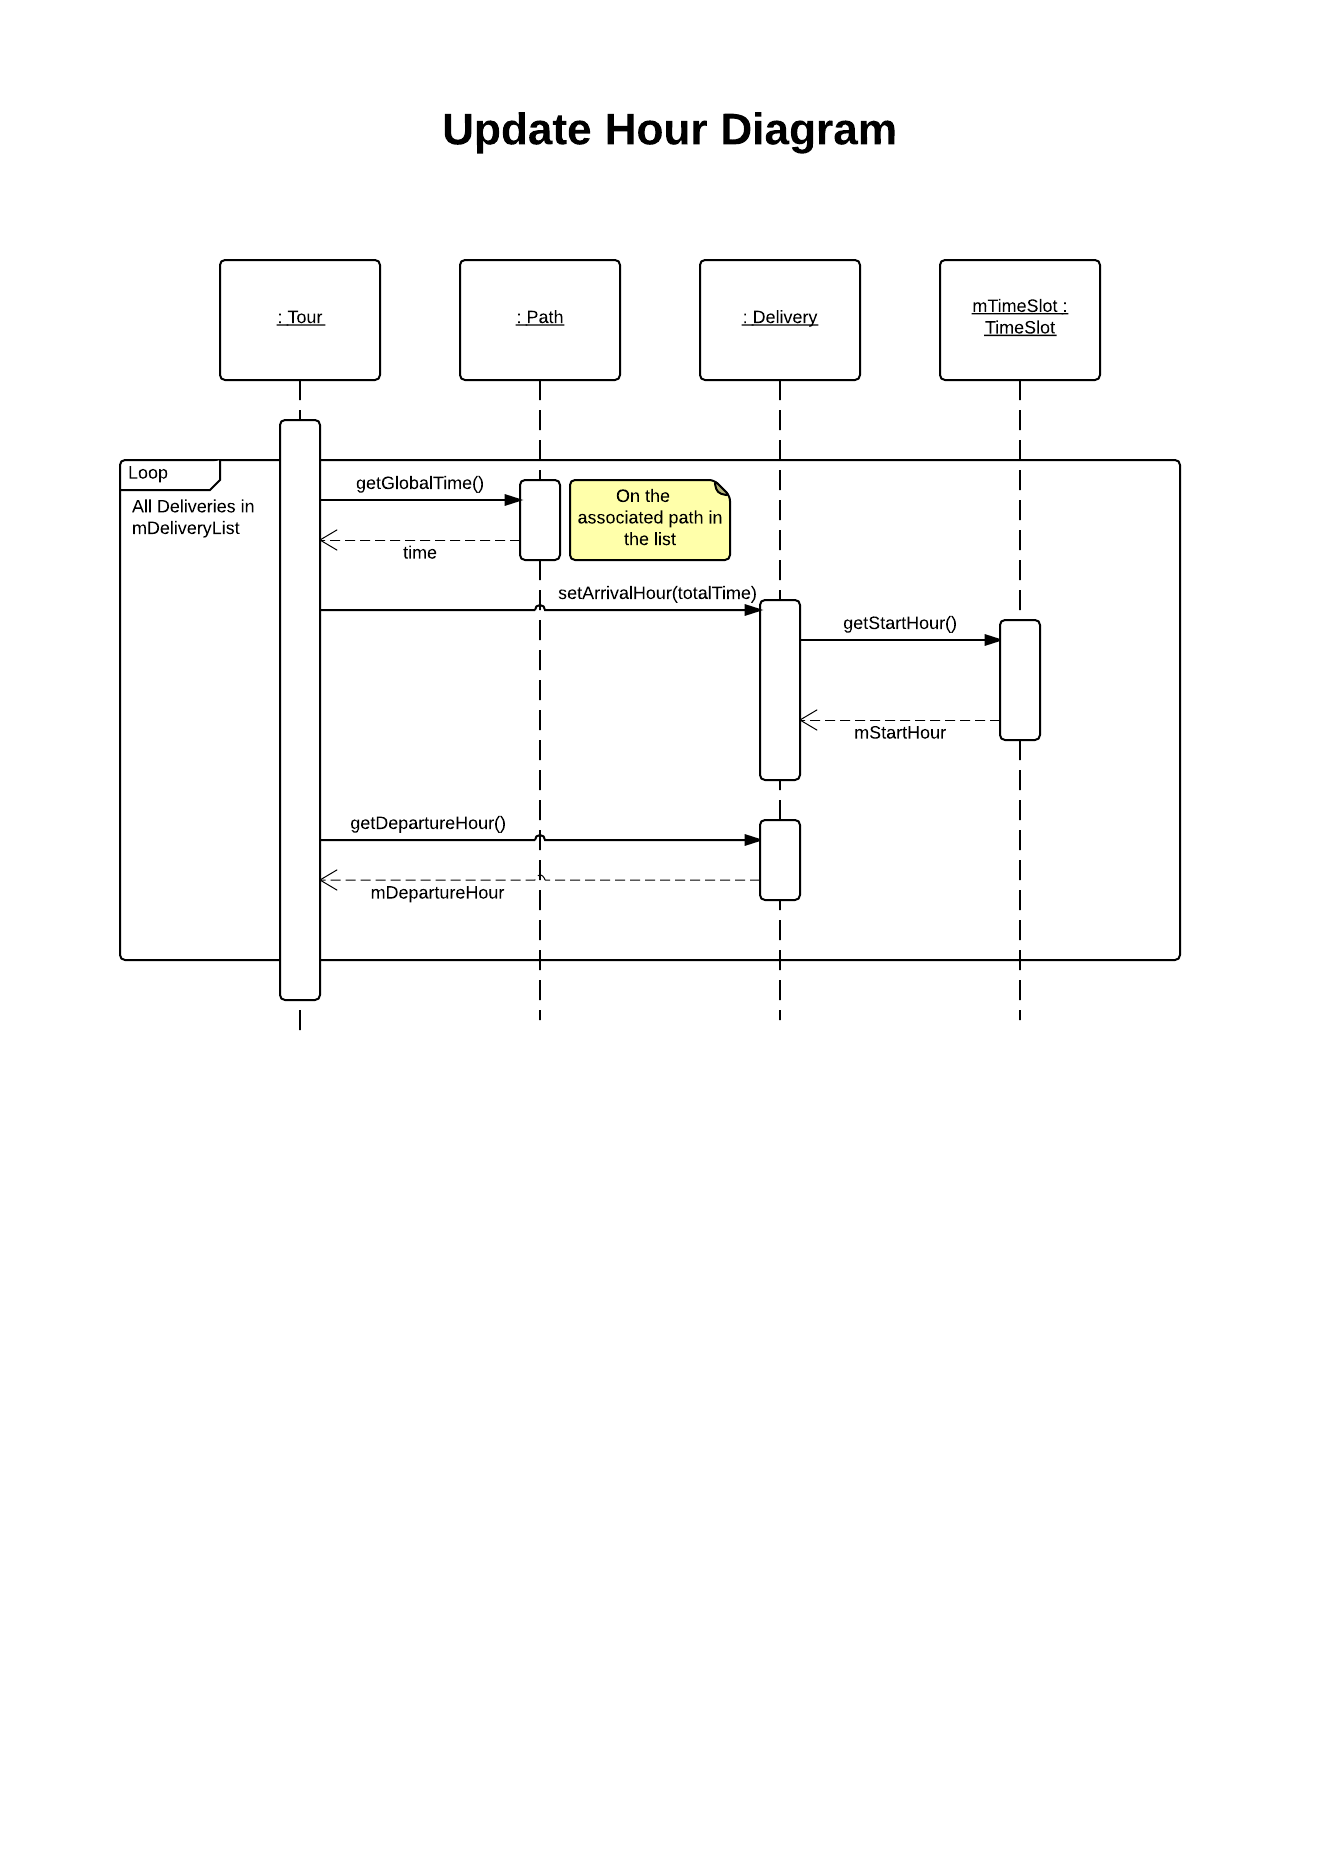
\includegraphics[width=\textwidth,height=\textheight,keepaspectratio, angle=90]{Figures/heure}
		\rule{35em}{0.5pt}
	\caption[Mise à jour de l'heure de livraison]{Mise à jour de l'heure de livraison}
\end{figure}


\subsection{Insertion d'un point de livraison dans une demande de livraison}

\begin{figure}[H]
	\centering
		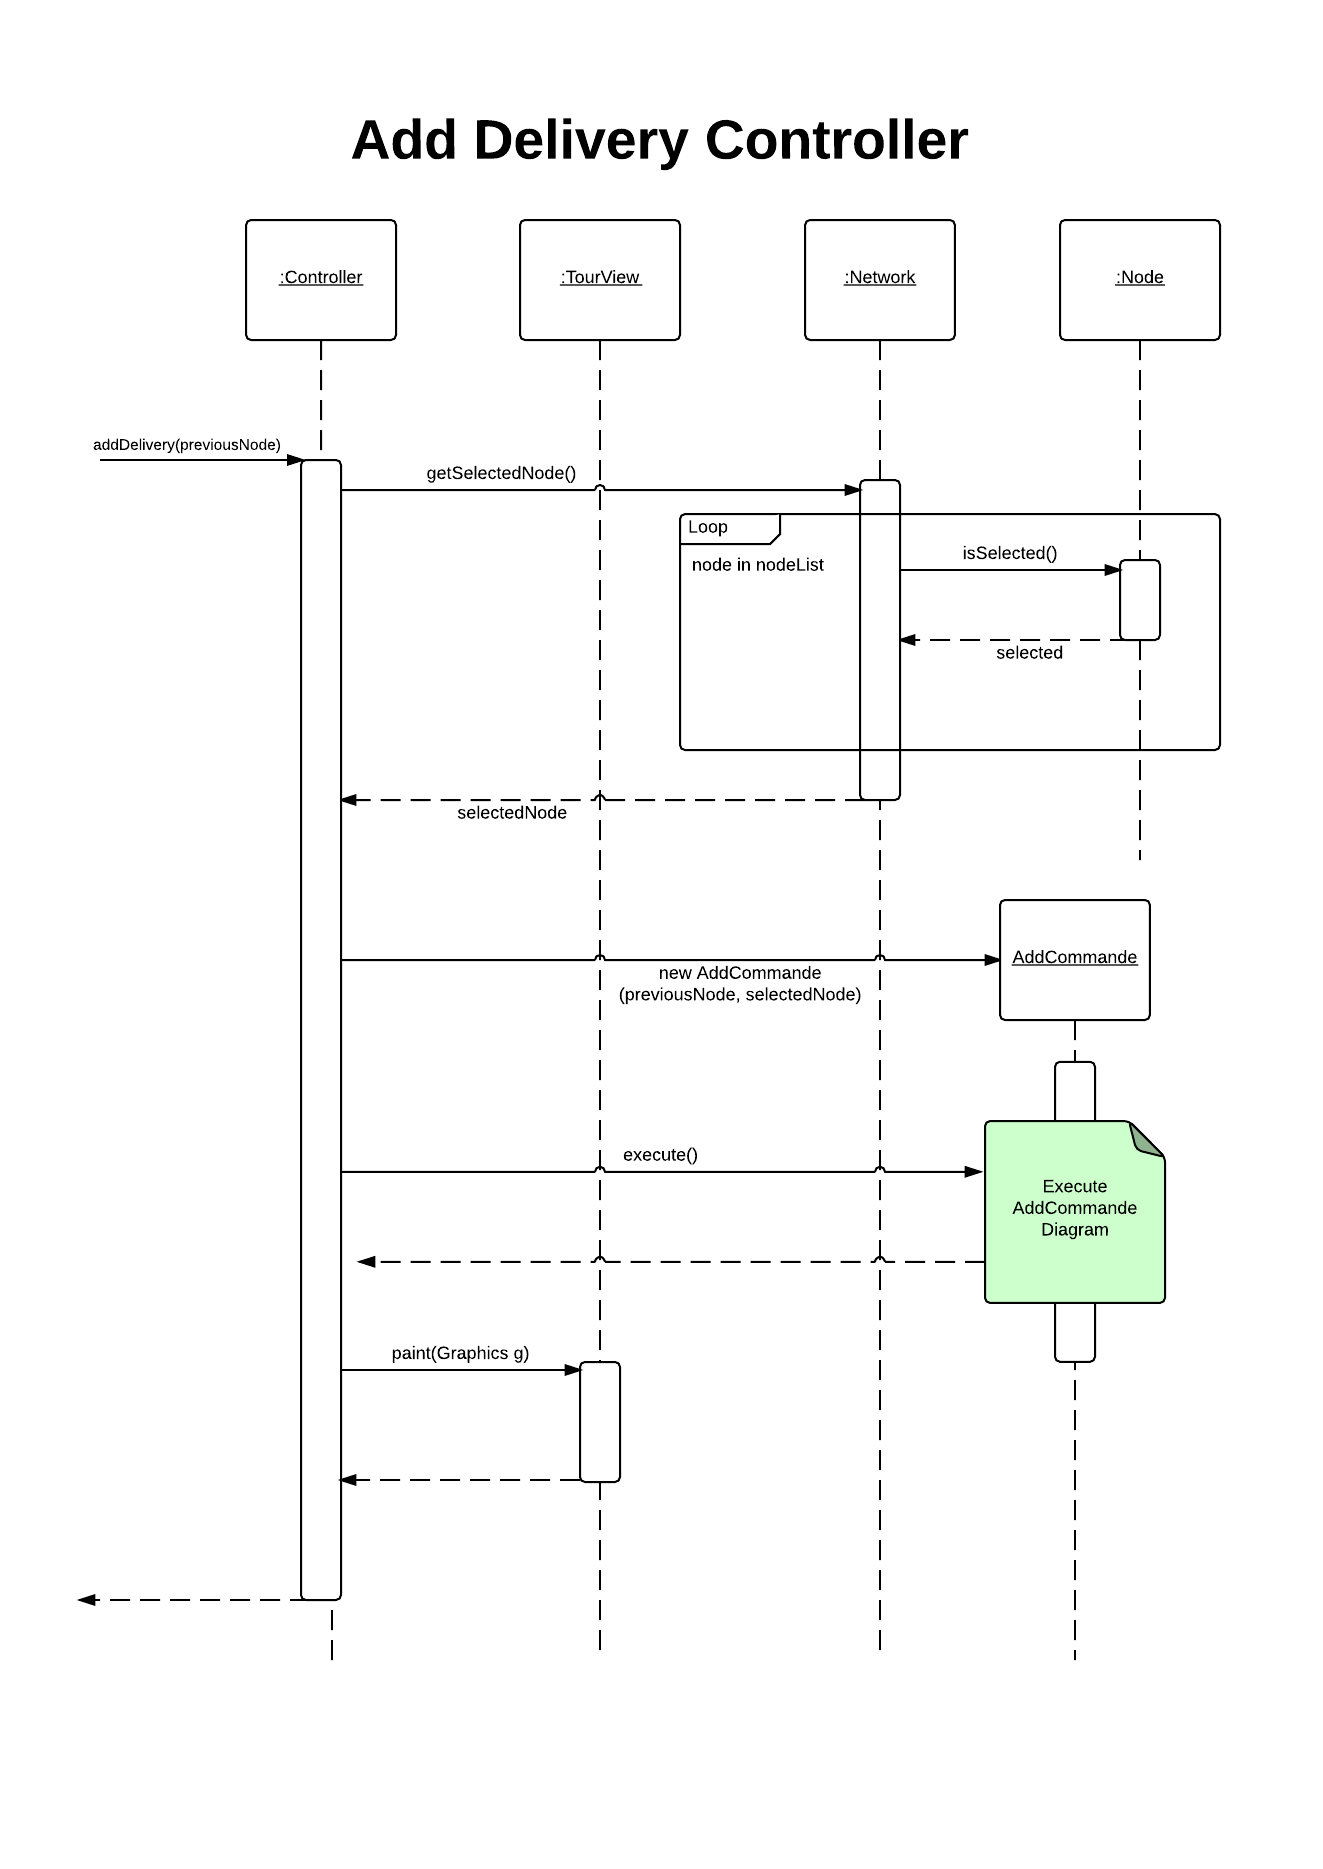
\includegraphics[width=\textwidth,height=\textheight,keepaspectratio]{Figures/ajout_livraison1}
		\rule{35em}{0.5pt}
	\caption[Ajout d'une livraison - diagramme général]{Ajout d'une livraison - diagramme général}
\end{figure}
\clearpage
\begin{figure}[H]
	\centering
		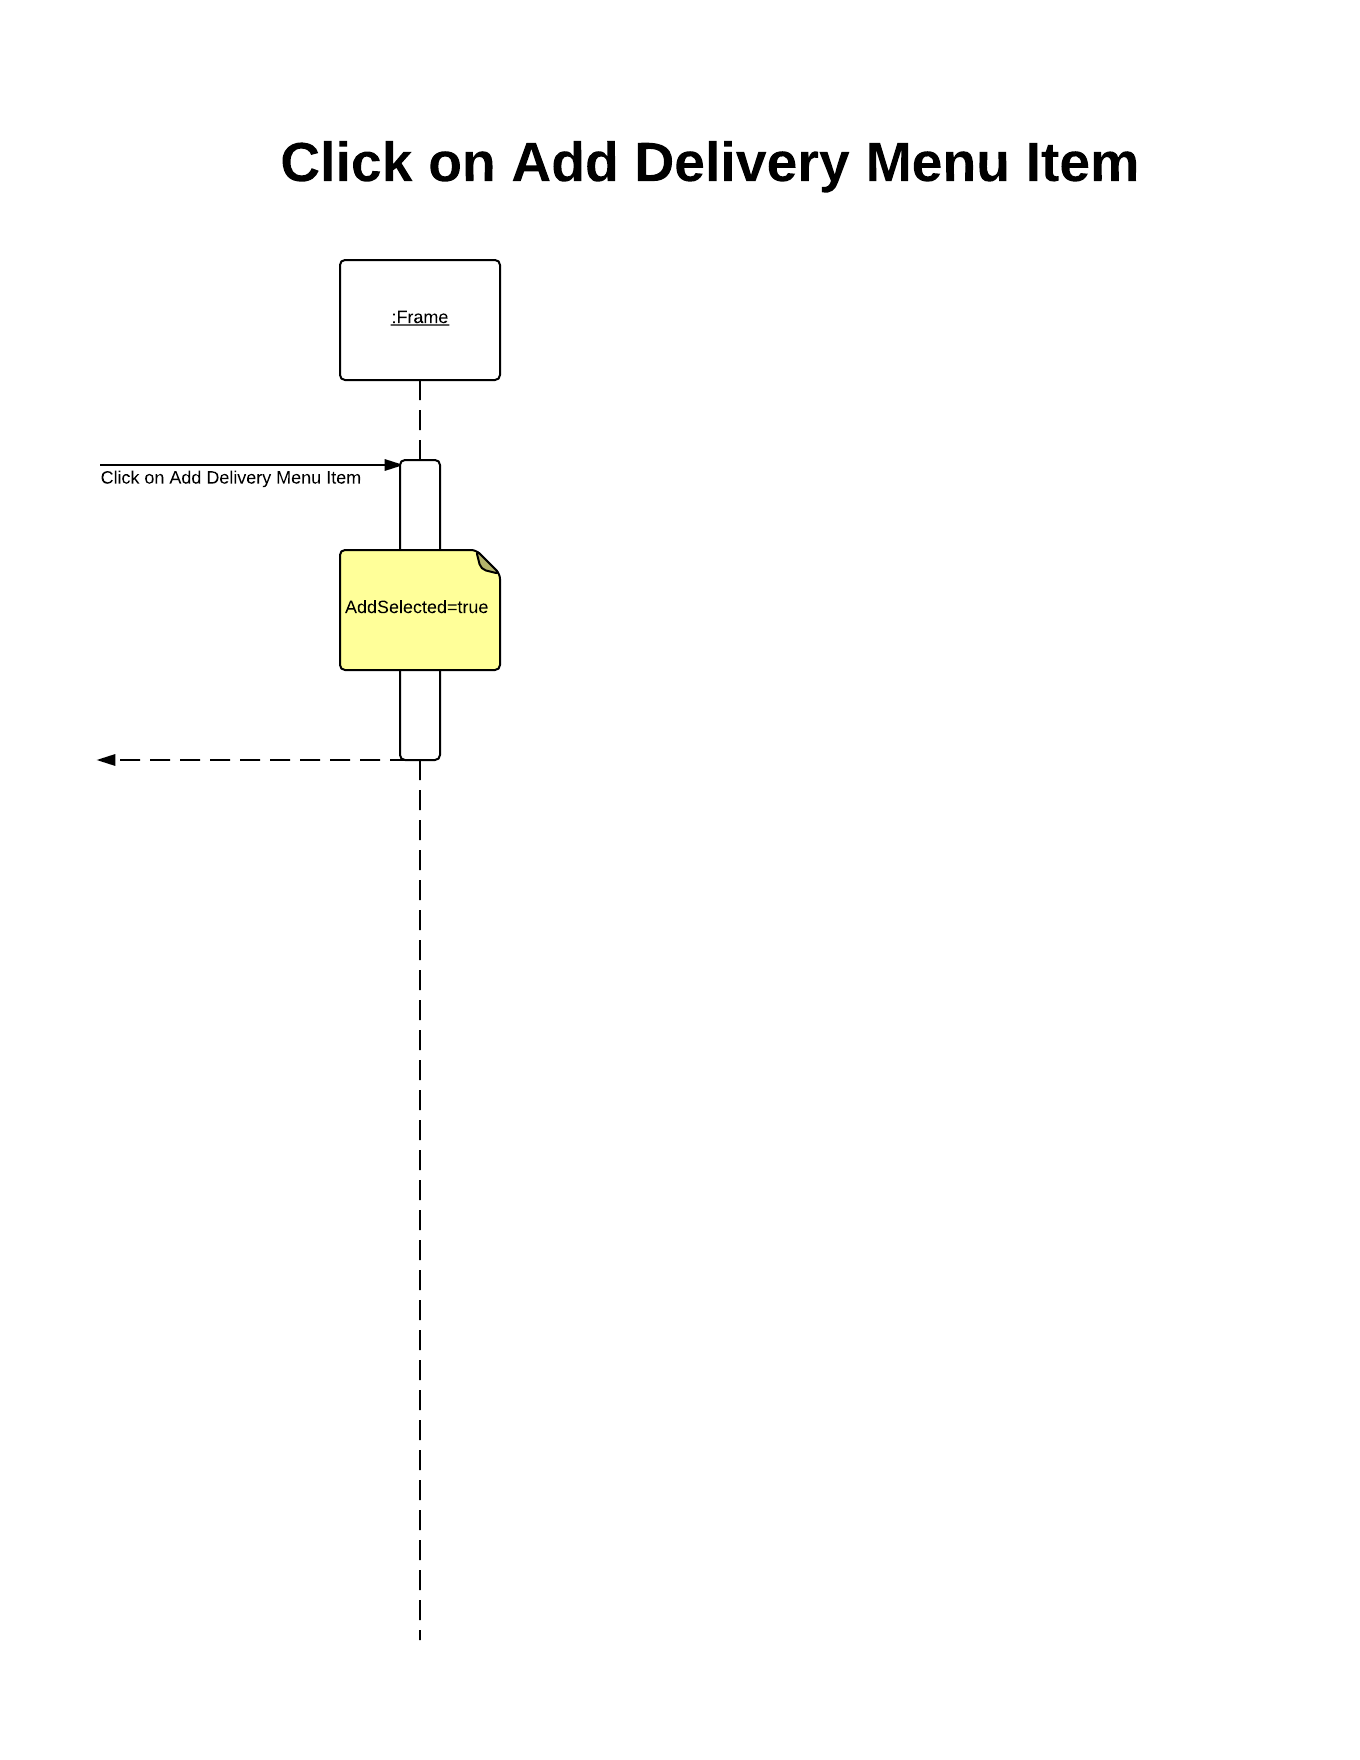
\includegraphics[width=\textwidth,height=\textheight,keepaspectratio]{Figures/ajout_livraison2}
		\rule{35em}{0.5pt}
	\caption[Click sur le menu]{Click sur le menu}
\end{figure}

\clearpage
\begin{figure}[H]
	\centering
		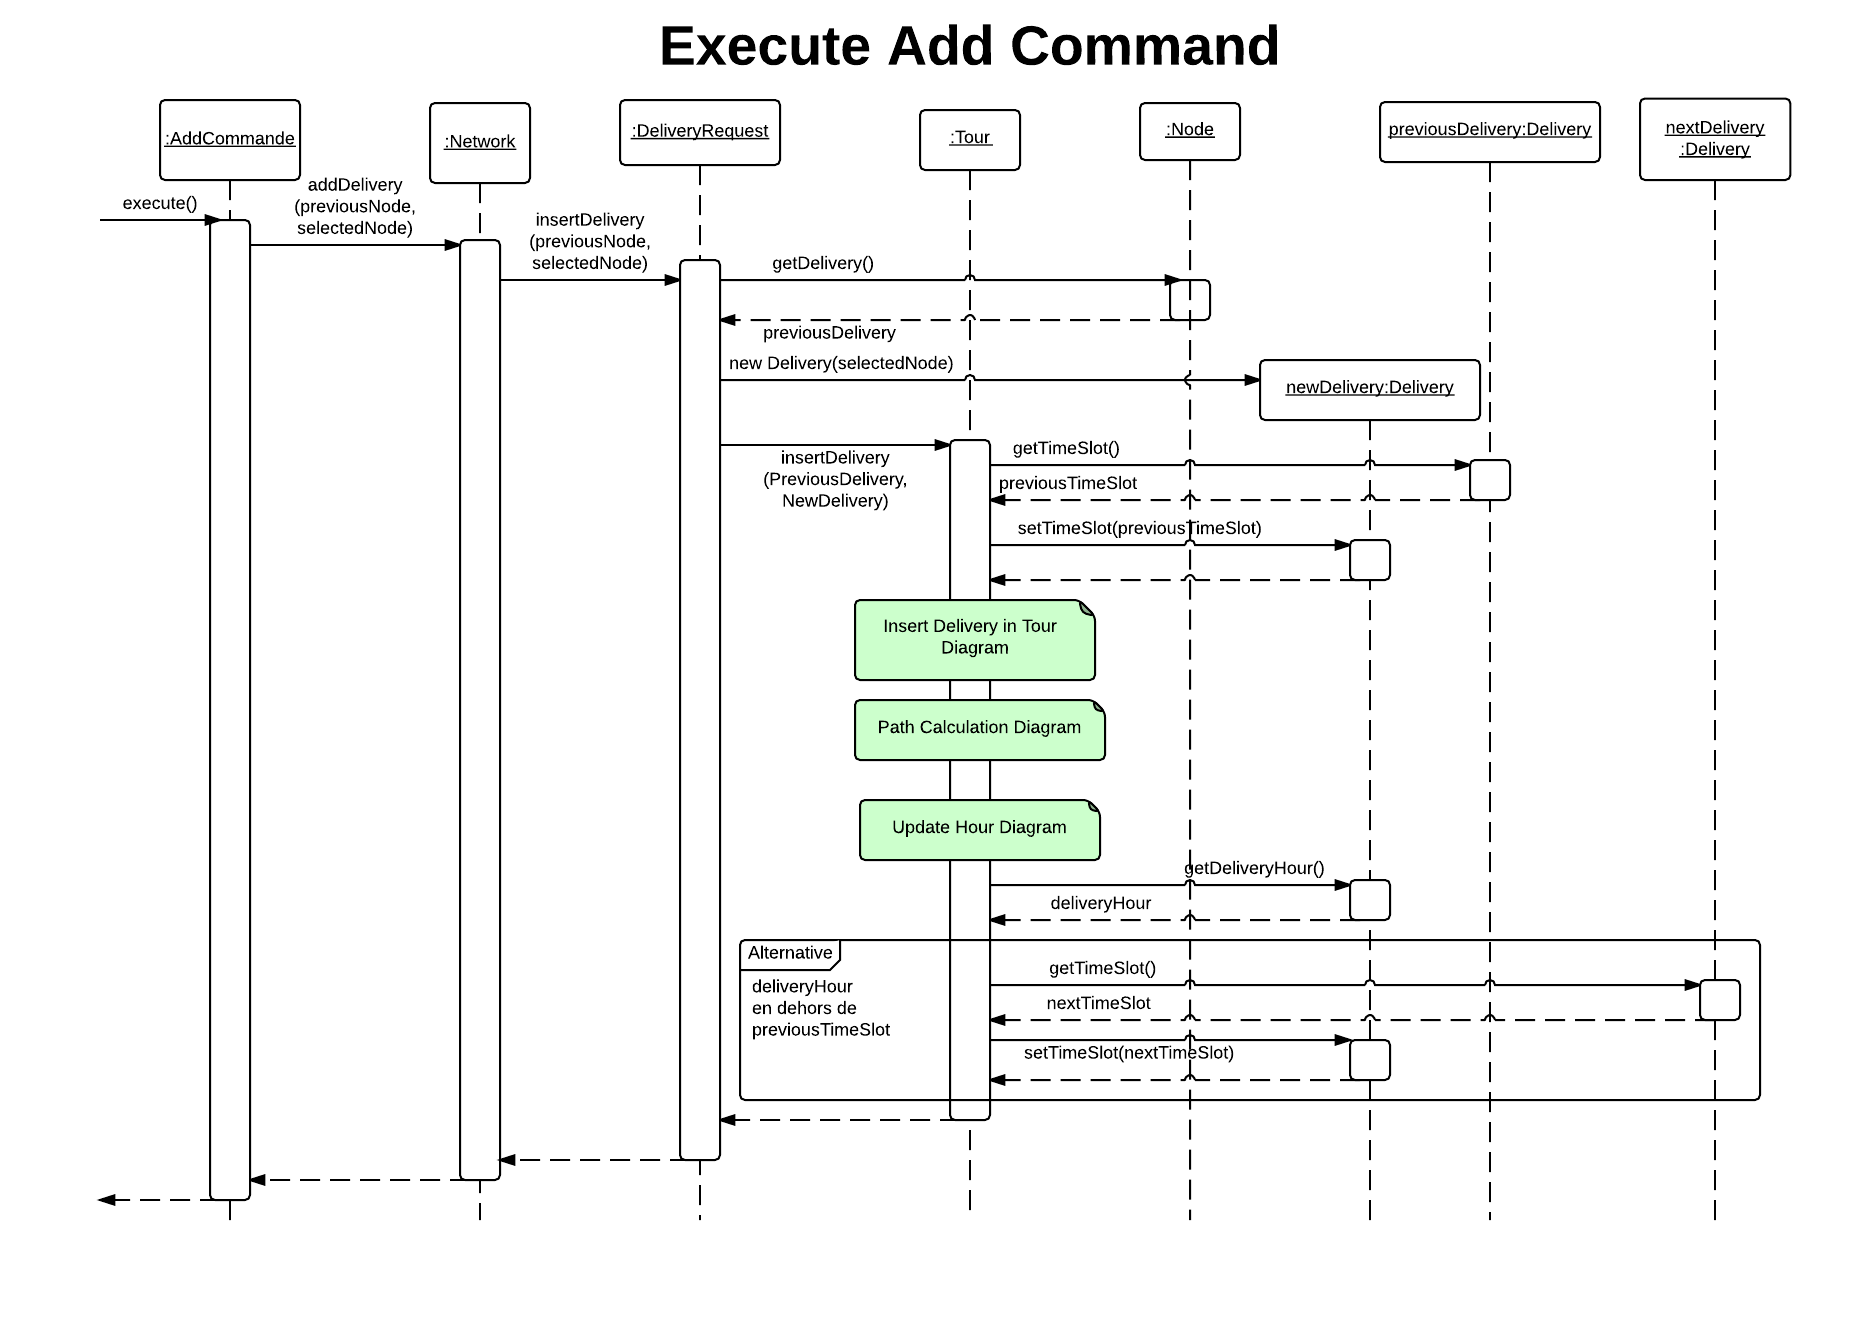
\includegraphics[width=\textwidth,height=\textheight,keepaspectratio, angle=90]{Figures/ajout_livraison3}
		\rule{35em}{0.5pt}
	\caption[Exécution de la commande Add]{Exécution de la commande Add }
\end{figure}

\clearpage
\begin{figure}[H]
	\centering
		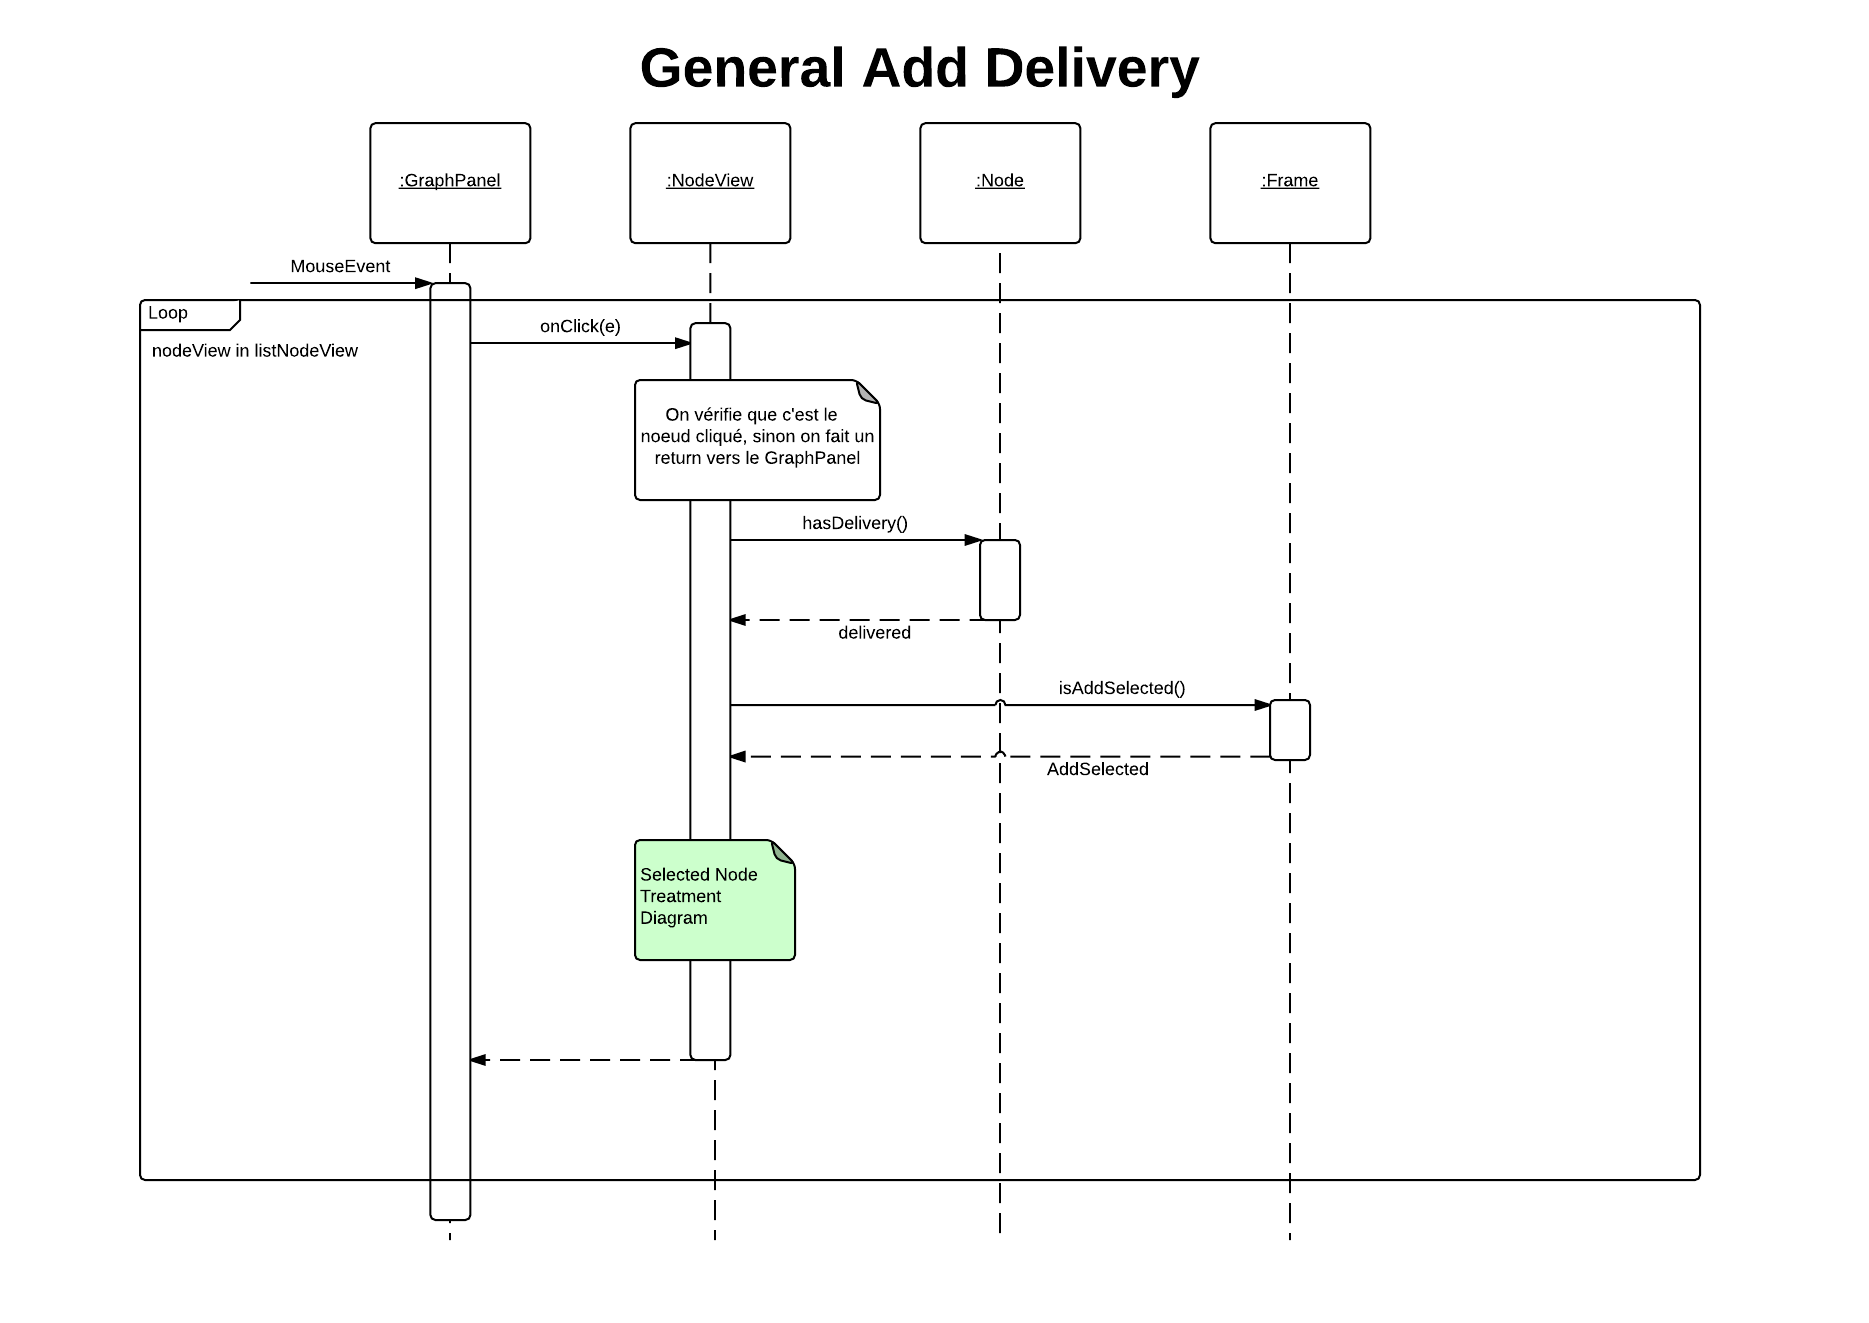
\includegraphics[width=\textwidth,height=\textheight,keepaspectratio, angle=90]{Figures/ajout_livraison4}
		\rule{35em}{0.5pt}
	\caption[Ajout d'une livraison]{Ajout d'une livraison}
\end{figure}

\begin{figure}[H]
	\centering
		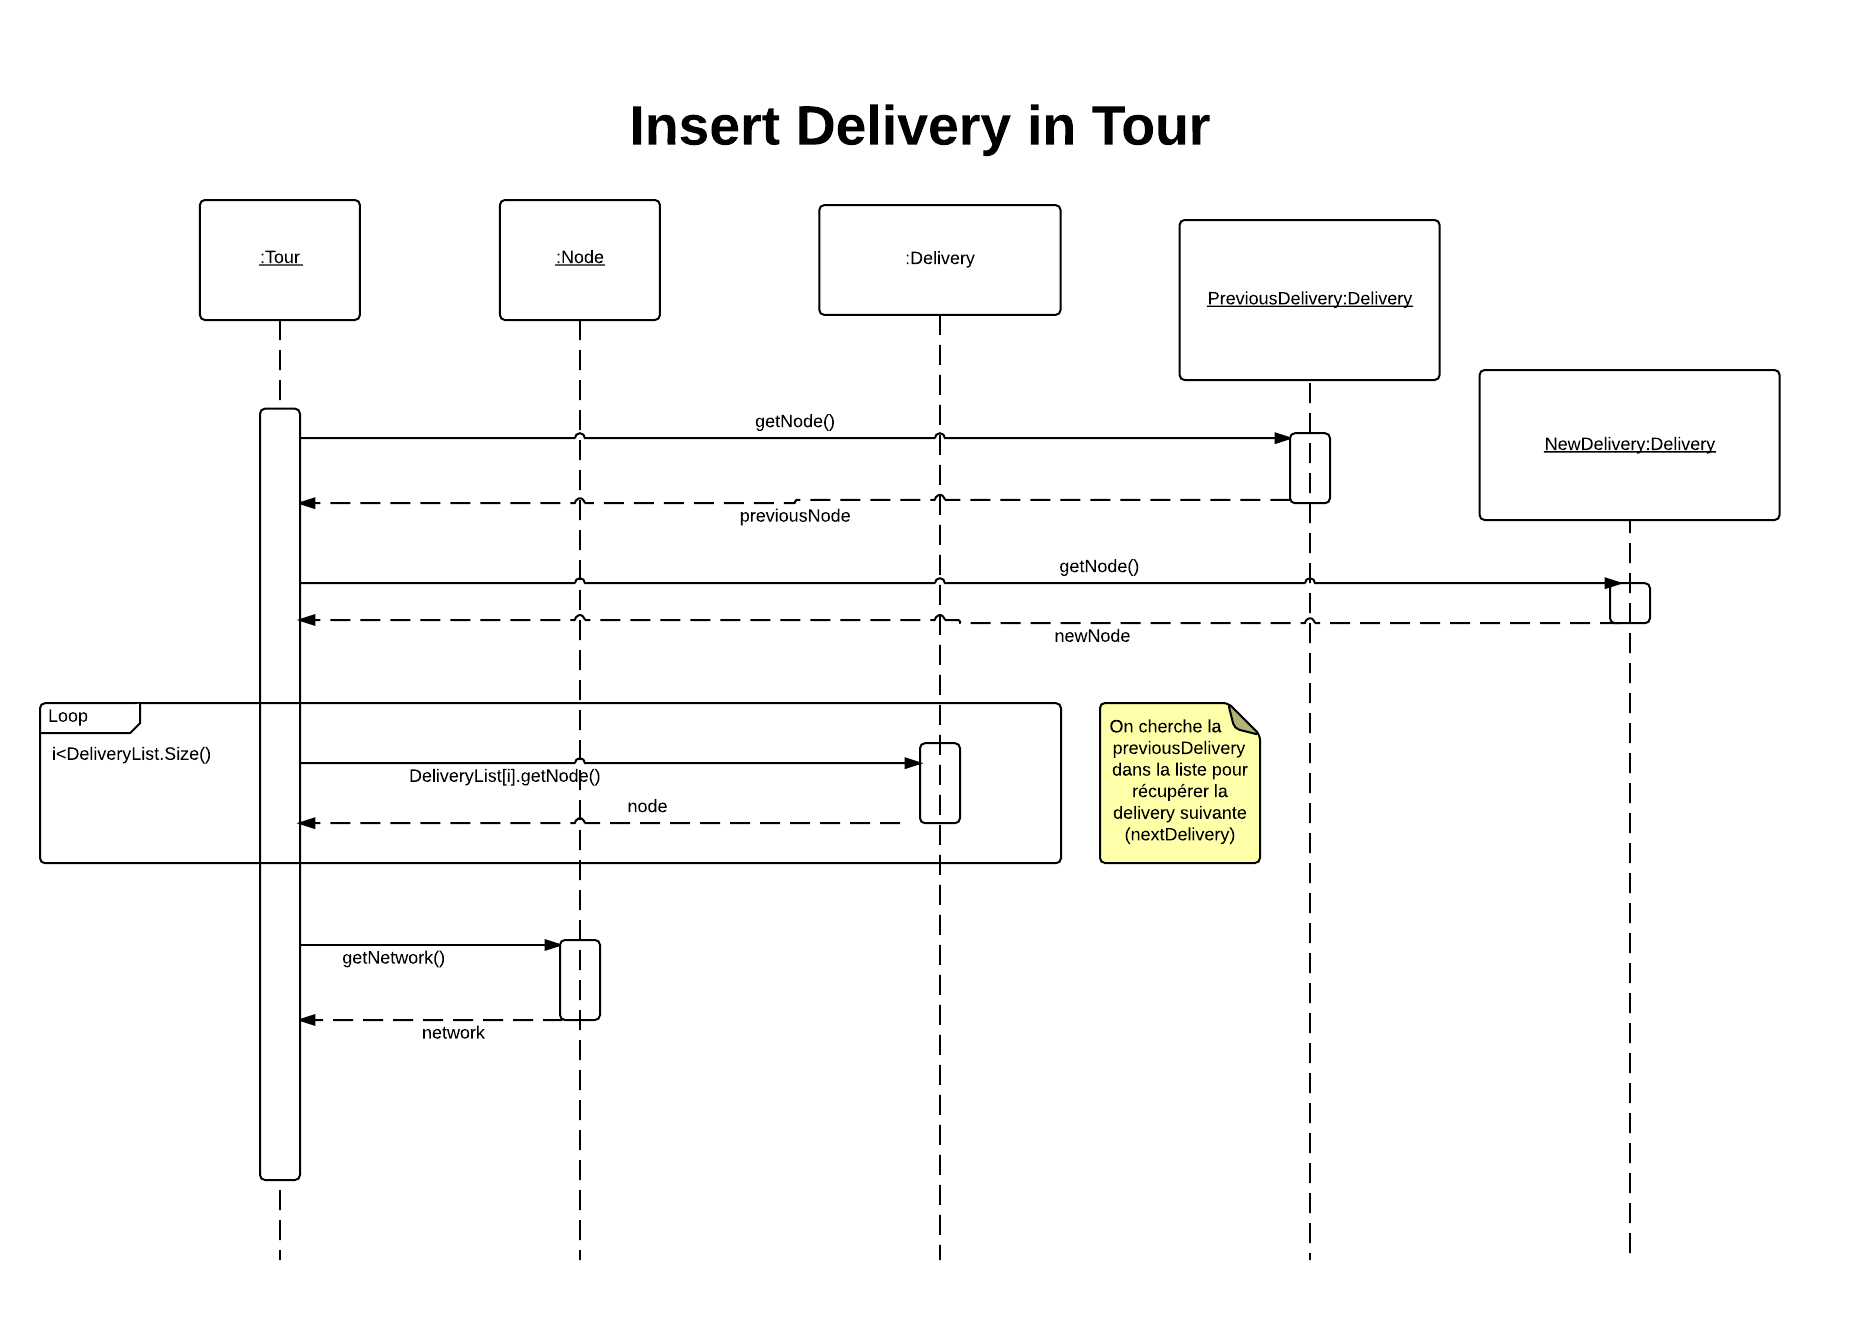
\includegraphics[width=\textwidth,height=\textheight,keepaspectratio, angle=90]{Figures/ajout_livraison5}
		\rule{35em}{0.5pt}
	\caption[Insertion d'une livraison dans la tournée]{Insertion d'une livraison dans la tournée}
\end{figure}


\begin{figure}[H]
	\centering
		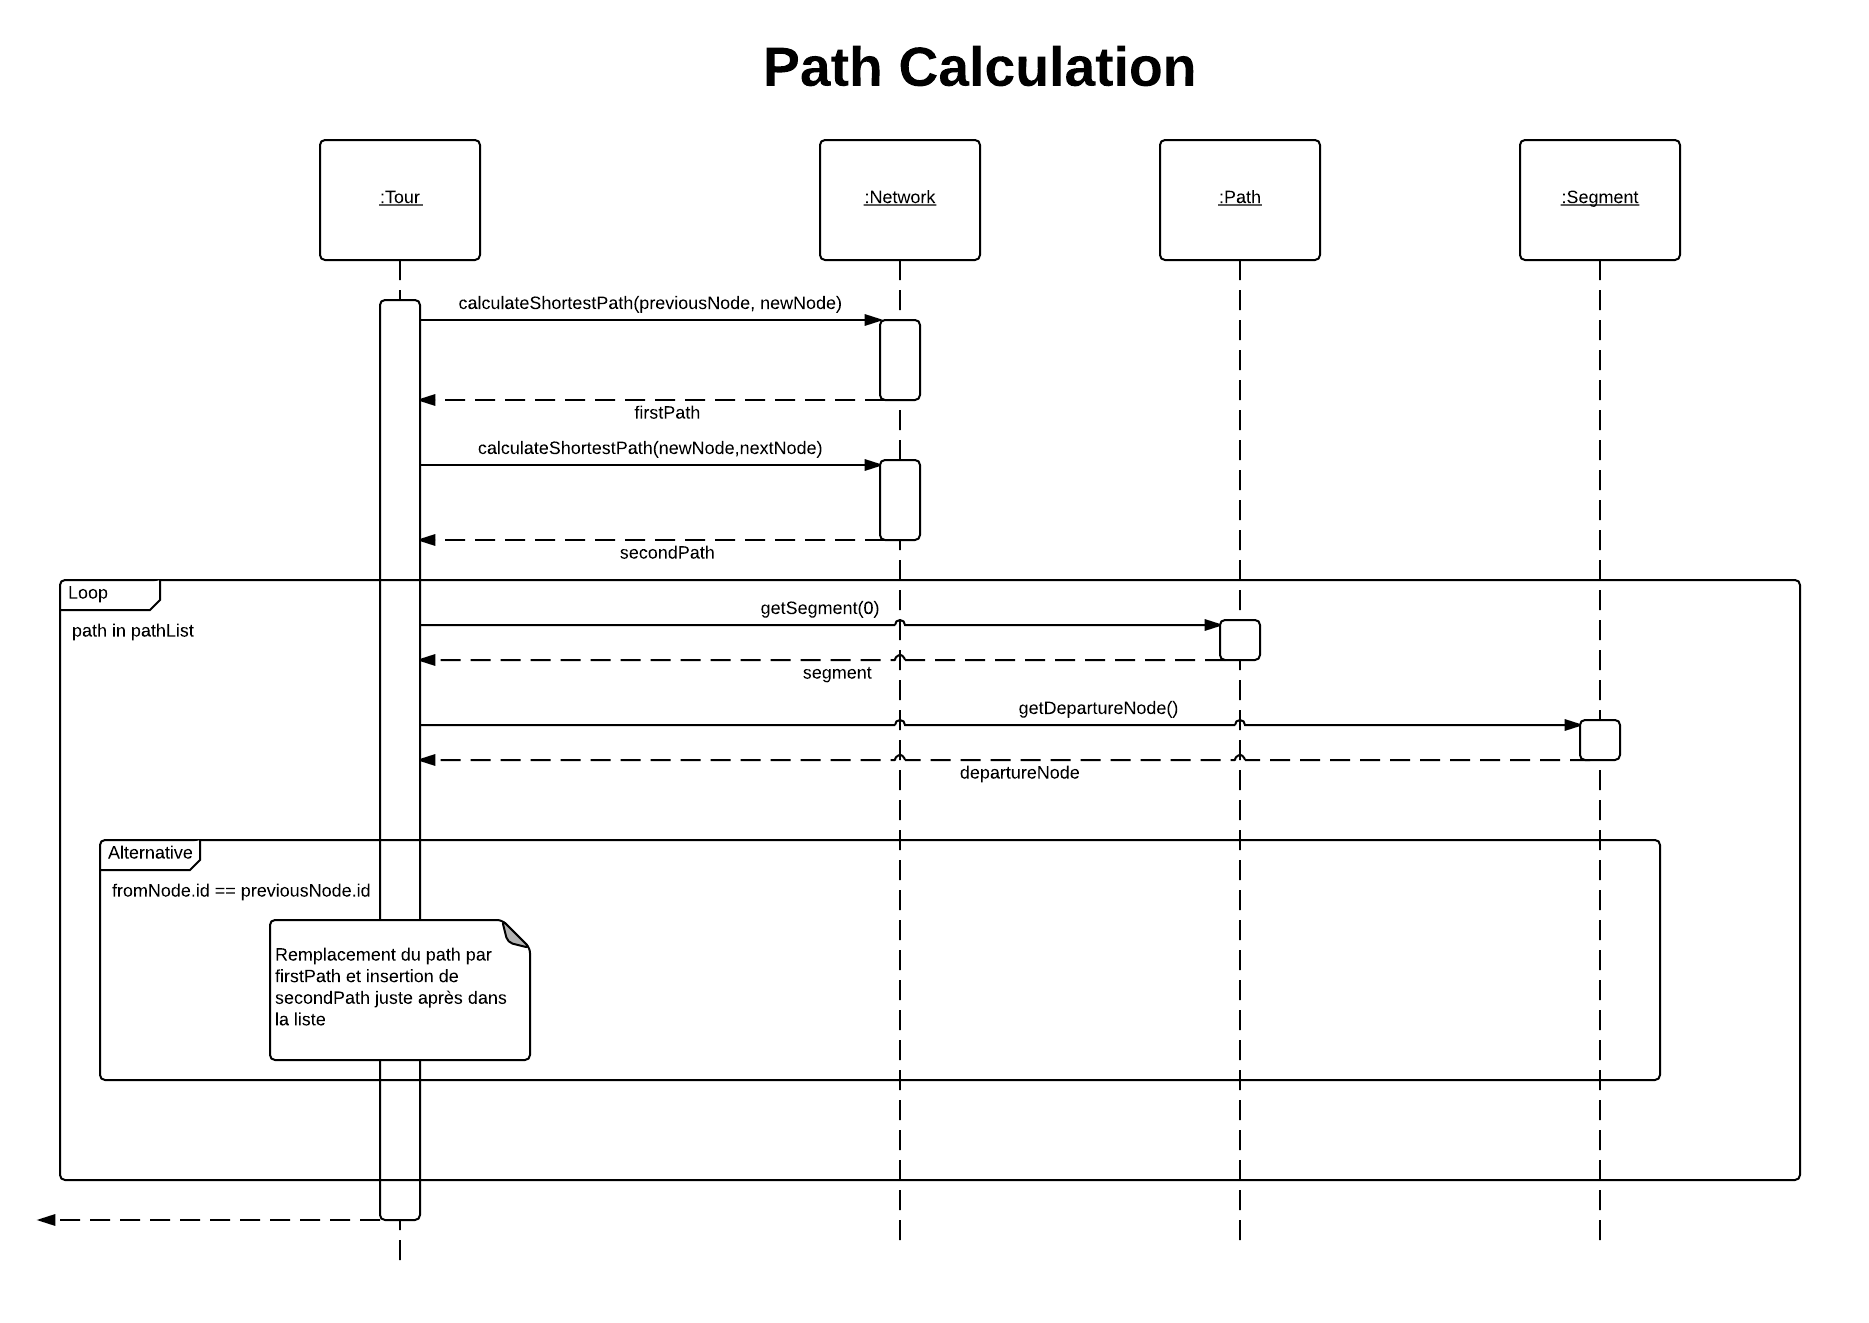
\includegraphics[width=\textwidth,height=\textheight,keepaspectratio, angle=90]{Figures/ajout_livraison6}
		\rule{35em}{0.5pt}
	\caption[Calcul du plus court chemin]{Calcul du plus court chemin}
\end{figure}

\begin{figure}[H]
	\centering
		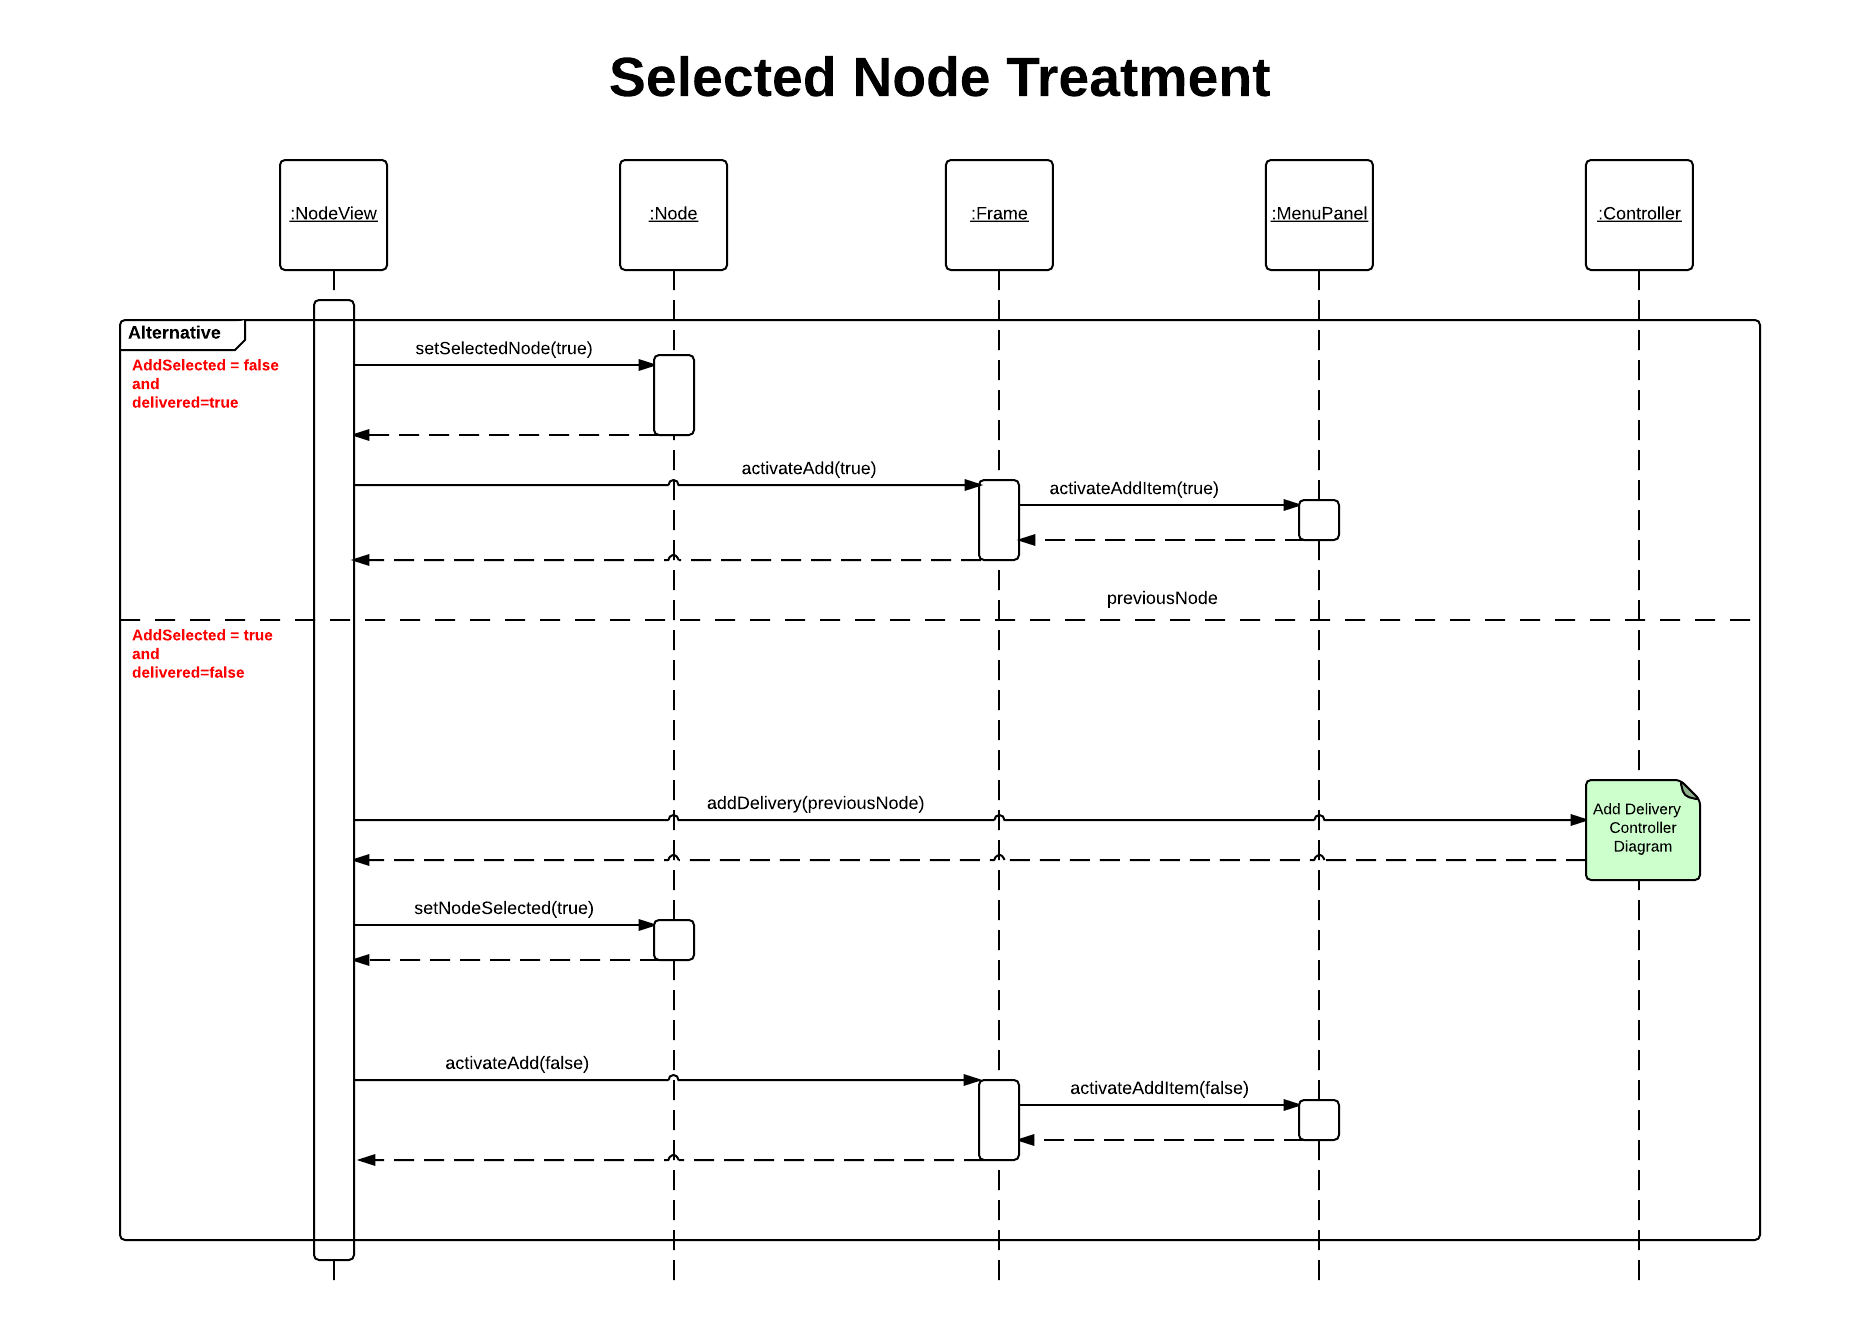
\includegraphics[width=\textwidth,height=\textheight,keepaspectratio, angle=90]{Figures/ajout_livraison7}
		\rule{35em}{0.5pt}
	\caption[Traitement du nœud sélectionné]{Traitement du nœud sélectionné}
\end{figure}
